\documentclass[runningheads]{llncs}
\bibliographystyle{splncs04}
\usepackage[T1]{fontenc}
\usepackage[misc]{ifsym}
\usepackage{graphicx}
\usepackage{array}


% = = = = = Packages = = = = = %

% !TEX root = ../main.tex

\usepackage{wrapfig}
\usepackage{tabularx}

% !TEX root = ../main.tex

% = = = Editing
\usepackage{xcolor}
\newcommand{\textblue}[1]{\textcolor{blue}{#1}}

% = = = Latin Short-Forms
\usepackage{xspace}
\newcommand{\etal}{\textit{et al.}\xspace}
\newcommand{\etc}{\textit{etc.}\xspace}
\newcommand{\ie}{\textit{i.e.,}\xspace}
\newcommand{\eg}{\textit{e.g.,}\xspace}
\newcommand{\cf}{\textit{cf.}\xspace}
\newcommand{\supra}{\textit{Supra}\xspace}
\newcommand{\nee}{\textit{n\'ee}\xspace}
\newcommand{\circa}{\textit{ca.}\xspace}
\newcommand{\aka}{\textit{a.k.a.}\xspace}
\newcommand{\cn}{\textblue{[cite]}}

% = = = Systems and Keywords
\newcommand{\kw}[1]{\textsf{#1}}
\newcommand{\polymarket}{\textsf{Polymarket}\xspace}
\newcommand{\truthcoin}{\textsf{Truthcoin}\xspace}
\newcommand{\gnosis}{\textsf{Gnosis}\xspace}
\newcommand{\augur}{\textsf{Augur}\xspace}

\newcommand{\depm}{DePM\xspace}
\newcommand{\cepm}{CePM\xspace}
\newcommand{\depms}{DePMs\xspace}
\newcommand{\cepms}{CePMs\xspace}

% = = =. URLs

\newcommand{\polyurl}[2]{Polymarket: `\href{#2}{#1}'}


% = = = Math
\newcommand{\lt}{$\rightarrow$\xspace}
\newcommand{\tuple}[1]{\left \langle #1 \right \rangle}

% = = = Crypto
\newcommand{\Zp}{\mathbb{Z}^{*}_{p}}
\newcommand{\Zq}{\mathbb{Z}_{q}}
\newcommand{\Gq}{\mathbb{G}_{q}}
\newcommand{\Enc}[1]{\mathsf{Enc}(#1)}
\newcommand{\EncB}[1]{\llbracket #1 \rrbracket}
\newcommand{\ReRand}[1]{\mathsf{ReRand}(#1)}
\newcommand{\Hash}[1]{\mathcal{H}(#1)}
\newcommand{\Sign}[1]{\mathsf{Sig}(#1)}
\newcommand{\Comm}[1]{\mathsf{Comm}(#1)}
\newcommand{\Open}[1]{\mathsf{Open}(#1)}







\usepackage{amsmath}
\usepackage{amssymb}
\usepackage{multirow}
\usepackage{tikz}
\usetikzlibrary{positioning,backgrounds}
\usetikzlibrary{trees}
\usepackage{hyperref}
\usepackage{tablefootnote}

%\usepackage{tabularx}
%\usepackage{array}
\usepackage{wasysym} 
\usepackage{ragged2e}
%\usepackage{float}

\usepackage{adjustbox}
\newcommand{\headrow}[1]{\multicolumn{1}{c}{\adjustbox{angle=45,lap=\width-0.5em}{#1}}}
\newcommand{\flatrow}[1]{\multicolumn{1}{c}{{#1}}}


% = = = = = Title = = = = = %

\begin{document}

\title{ SoK: Market Microstructure for Decentralized Prediction Markets (\depms)}

\author{
	Nahid Rahman\inst{1} \and 
	Joseph Al-Chami\inst{2}\orcidID{0009-0001-8381-8080} \and 
	Jeremy Clark\inst{1}\orcidID{0000-0002-3533-5965}
	}

\institute{
	Concordia University, Montreal, Canada \\ \email{nahid.rahman@mail.concordia.ca} \\ \email{j.clark@concordia.ca} \and
        Independent Researcher \\ \email{alchamijoseph@gmail.com}
	}
	

\maketitle


% = = = = = Abstract = = = = = %

% !TEX root = ../main.tex
\begin{abstract}

Decentralized prediction markets (\depms) allow open participation in event-based wagering without fully relying on centralized intermediaries. We review the history of \depms which date back to 2011 and includes hundreds of proposals. Perhaps surprising, modern \depms like Polymarket deviate materially from earlier designs like Truthcoin and Augur v1. We use our review to present a modular workflow comprising seven stages: underlying infrastructure, market topic, share structure and pricing, trading, market resolution, settlement, and archiving. For each module, we enumerate the design variants, analyzing trade-offs around decentralization, expressiveness, and manipulation resistance. We also offer open problems for researchers interested in contributing to this ecosystem.

\end{abstract}
%\keywords{security \and cryptography}

% = = = = = Main Body = = = = = %

% !TEX root = ../main.tex
\section{Introduction}

In late 2024, the United States was in the midst of a presidential election when the decentralized prediction market, Polymarket~\cite{poly}, broke through mainstream news coverage~\cite{Cha24,YBG24a}. Stories focused, in particular, on the fact that it offered odds more favourable to eventual winner Donald Trump than those reflected in conventional polls and forecasts. Polymarket's odds are not set by experts or pundits, instead it is a specific type of betting market where odds are extrapolated from the prices of trades made in an open market (or somewhat open, as Polymarket was banned at the time in many countries including the US). 

As with traditional betting, whether online or through a bookie, prediction markets allow speculators to profit from correct forecasts~\cite{AFGH+08,WoZi06}. However the structure of a prediction market is different than traditional betting. One key difference is that prediction markets ease the process of moving in and out of bets before the event resolves, encouraging traders to place bets if they think the odds are over- or under-stated, and withdrawing profits if the odds realign.

It would be easy to think that Polymarket's design is the most obvious, straight-forward way to deploy a decentralized prediction market (\depm) on a blockchain. However the central thesis of this systemization of knowledge (SoK) paper is that Polymarket found success in bucking the trend. \depms were first given a few paragraphs in the Ethereum vision paper~\cite{But13}, released in late 2013 for the blockchain that would be deployed in 2015. Then two 2014 papers presented flushed out systems: a whitepaper called Truthcoin~\cite{Sz14} and an academic paper at WEIS 2014~\cite{BCFKMN14} (informally known as the `Princeton \depm' because of author affiliation). Developed independently,\footnote{The Princeton paper describes Truthcoin as being released while the paper was under review~\cite{BCFKMN14}, and the Truthcoin FAQ~\cite{Sz14b} mentions hearing about the Princeton paper but not having found the paper itself.} the two papers' designs are vastly different, representing two different goalposts for how a \depm might look. 

Early systems, like Augur~\cite{AKPWZ15} and Gnosis~\cite{Gn17} closely resembled Truthcoin~\cite{Sz14}, while modern systems like Polymarket~\cite{poly} either resemble the Princeton \depm~\cite{BCFKMN14} or use new solutions that resemble a hybrid of the two designs. Consider some examples:

\begin{enumerate}
\item From \S\ref{wf:price}, in Truthcoin, the market creator is active in setting initial prices (\ie odds) for each option and risks its own money (bounded)~\cite{Sz14}. In the Princeton system, the market creator is passive, not setting prices or risking any money~\cite{BCFKMN14}. Polymarket uses the latter~\cite{poly}. 

\item From \S\ref{wf:trade}, in Truthcoin, outcome shares are created with predecessor to an automated market maker~\cite{Sz14}. In the Princeton \depm, outcome shares are traded with an orderbook~\cite{BCFKMN14}. In Polymarket, outcome shares can be traded with either an AMM or an orderbook~\cite{poly}. 

\item From \S\ref{wf:close}, in Truthcoin, the blockchain decides event outcomes (\eg who won the election) through a reputation-based on-chain vote with slashing~\cite{Sz14}. In the Princeton paper, they are resolved through trusted arbiters acting as oracles~\cite{BCFKMN14}. The Ethereum whitepaper suggests both~\cite{But13}. In Polymarket, the third party oracle, UMA, operates under the hood through on-chain voting with slashing, but only when outcomes are disputed~\cite{poly,uma}.
\end{enumerate}

Noticing these points of differences inspired us to ask what are all the design decisions involved in creating a \depm?  We reviewed over a hundred projects, distilled into the 35+ notable \depms listed in Appendix~\ref{app:list}. From these, we break the \depm design space into a `modular workflow' (the method used in an SoK at AFT 2021 on oracles~\cite{ClEsGS21}) with seven stages: underlying infrastructure, market topic, share structure and pricing, trading, market resolution, settlement, and archiving. For each stage, we enumerate the possible designs and discuss competing trade-offs. 

% ChatGPT generated timeline so cross-validate everything before believing any of it:
%	•	1988 — Iowa Electronic Markets (IEM) launch as an academic, real-money prediction market at the University of Iowa.   
%	•	1990–2003 — Robin Hanson foundation work: “Idea Futures” concept (1990s) and the logarithmic market scoring rule (LMSR) (2002/03), which becomes the standard automated market maker design for PMs.  
%	•	2003 — Policy Analysis Market (PAM) (DARPA) announced then quickly canceled amid controversy; keeps prediction markets in the policy spotlight.   
%	•	2012–2013 — Intrade exits U.S. and then shuts down following a CFTC lawsuit (Nov 26, 2012) and subsequent turmoil (site shutdown Mar 10, 2013).    
%	•	2013–2014 — Ethereum vision includes prediction markets as a core smart-contract use case.  
%	•	2014 — Princeton/WEIS paper “On Decentralizing Prediction Markets and Order Books” sketches a Bitcoin-based design; a seminal academic reference for on-chain PMs.  
%	•	2014–2015 — Truthcoin / Hivemind (Paul Sztorc) proposes a Bitcoin sidechain oracle + PM protocol (whitepaper v1.5 dated Dec 2015; early drafts 2014).   
%	•	2015 — Augur token sale (~$5M) to build a decentralized oracle + PM on Ethereum.  
%	•	2016–2017 — Gnosis forms & conducts ICO (2017) to pursue PMs and related tooling on Ethereum.  
%	•	2018 — Augur v1 goes live on Ethereum (first major decentralized PM on mainnet).  
%	•	2018 — Kleros launches (Ethereum-based decentralized court), later widely used with Reality.eth as an oracle stack for PM-style applications.   
%	•	2020 — Augur v2 launches (DAI-denominated, faster resolution; “Invalid” tradable), marking a big UX/market-mechanics upgrade.  
%	•	2020 — Omen (by Gnosis) launches a PM front-end using the Conditional Tokens Framework on xDai/Gnosis Chain.  
%	•	2020 — Polymarket launches and grows rapidly; runs on Polygon PoS and (today) resolves via UMA’s Optimistic Oracle.   
%	•	2021 — Augur Turbo launches on Polygon with sports & rapid markets.  
%	•	2021–2024 — Zeitgeist launches as a PM parachain on Kusama and migrates to Polkadot in 2024.  
%	•	2022 — CFTC settles with Polymarket (geoblocks U.S. users; continues ex-U.S.).  
%	•	2020 onward — GnosisDAO experiments with futarchy, i.e., governance guided by prediction markets.   
%	•	2024 — U.S. appeals court clears Kalshi to offer election markets, a major regulatory milestone for event markets in the U.S. (not blockchain-based, but highly relevant).  

% = = = = = = = = = = = = = = = = = = = = = = = = = = = = = = = = = = = = = = = = = = = = = = = = 
 
\section{Preliminaries}

\subsection{Methodology}

We obtained a collection of academic works on decentralized prediction markets, as well as various intersecting topics including (centralized) prediction markets, oracles, DeFi, and AMMs. We used our knowledge of the field, Google Scholar (search and cited by features), and citations within papers. Our library is available, sorted by topic, on Zotero.\footnote{Zotero: \textblue{Link withheld for anonymity.}} We also identified projects without white-papers or academic papers, reviewing the 97 current projects listed on a recently released online dashboard~\cite{Sal25} (noting that some listed are \depm-adjacent rather than true \depms) and by studying 20+ historical systems that are no longer active. We also searched news sources for opinions and issues on leading decentralized prediction markets, such as Polymarket. We used affinity diagrams to cluster design decisions into the seven stages of our final modular framework. Relevant artifacts and data are available on GitHub.\footnote{GitHub: \textblue{Link withheld for anonymity.}}   

% = = = = = = = = = = = = = = = = = = = = = = = = = = = = = = = = = = = = = = = = = = = = = = = = 

\subsection{Taxonomy}

Consider the following taxonomy of a few wagering systems:

\adjustbox{max width=\textwidth}{
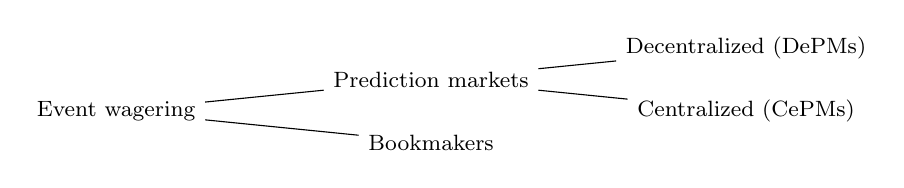
\begin{tikzpicture}[
  font=\footnotesize,
  grow=right,                    % horizontal (left -> right)
  level distance=40mm,           % horizontal gap between levels
  sibling distance=8mm,          % vertical gap between siblings
  box/.style={draw, rounded corners, align=left, inner sep=2pt, text width=28mm}
]
\node{Event wagering}
  child { node{Bookmakers} }
  child { node[]{Prediction markets}
    child { node[]{Centralized (\cepms) } }
    child { node[]{Decentralized (\depms)} }
  };
\end{tikzpicture}
}

\paragraph{Bookmakers versus prediction markets.}

A wager is a two-party contract with payouts based on the outcome of a future event. Consider Alice and Bob who wager on the same outcome of an event. With a fixed-odds bookmaker (or online betting), Alice's contract is different from Bob's contract in at least two regards: (i) it specifically names Alice as the counterparty and (ii) the payouts could be different if the odds changed between Alice's wager and Bob's. By contrast, in a prediction market contract (called a outcome share), Alice and Bob hold identical contracts: (i) all contracts are between the market operator and whoever redeems the contract, and (ii) the payout is exactly the same (typically \$0 if incorrect and \$1 if correct). Odds are reflected in the price paid for a prediction market contract (\ie variable cost and fixed payout), while a bookmaker contract has a fixed cost and variable payout. Thus the key distinction is that prediction market outcome shares are \textit{fungible} and can be freely traded between participants, enabling a free market that communicates information to the public through outcome share prices, trading volume, market depth, and other financial market metrics. Other wager structures include parimutuel betting~\cite{ThZi88,KNZ08,ULSM25}, back/lay exchanges~\cite{CHKL21} and cash for difference contracts~\cite{ACES17}.

\paragraph{\cepm versus \depm.}

The term \textit{decentralized prediction market} originates from the Ethereum whitepaper~\cite{But13} and we abbreviate it \depm to match terms like DeFi (decentralized finance)~\cite{WPG+22} and DePIN (decentralized physical infrastructure networks)~\cite{LWS+24,MEB+25}. The term \textit{decentralized}~\cite{OKK24} in each of these is actually shorthand for both \textit{decentralized} and \textit{permissionless}, where permissionlessness is generally the more important way \depms distinguish themselves from centralized prediction markets (\cepms). Permissionlessness could extend itself to the market topic, the trading of outcome shares, the closing of the market, and the withdrawing of rewards, but not all systems will open up each of these operations (as we will explain in \S\ref{sec:wf}). We say a system is \depm if at least one is permissionless.

 % = = = = = = = = = = = = = = = = = = = = = = = = = = = = = = = = = = = = = = = = = = = = = = = = 

\subsection{Definitions}
\label{sec:defn}

% !TEX root = ../main.tex

We define a market within a prediction-market system. In contrast to existing definitions, we abstract away details about how they are implemented. If the definitions are not clear, we refer the reader to Appendix~\ref{app:example} where we describe a specific market offered by Polymarket and map each term in the following definitions to this real world example.

\begin{definition}[Market]\label{def:market}
A (single) market is a tuple $M=(E,\Omega,J,R)$, where $E$ is a well-defined uncertain event, $\Omega$ is a nonempty outcome space for $E$, $J$ is a finite index set of contract labels (“shares”), and $R=(R_j)_{j\in J}$ are nonnegative payoff functions with $R_j:\Omega\to\mathbb{R}_{\ge 0}$. When $M$ resolves to $\omega_M\in\Omega$, one unit of share $j\in J$ pays $R_j(\omega_M)$ (in units of $\mathcal{N}$ defined below).
\end{definition}

\begin{definition}[Prediction--market system]\label{def:system}
A prediction--market system is a tuple $\mathcal{S}=(\mathcal{M},\mathcal{N},\mathsf{Res})$, where $\mathcal{M}$ is a countable set of markets, $\mathcal{N}$ is a numeraire (unit of account), and $\mathsf{Res}=\{\mathrm{res}_M\}_{M\in\mathcal{M}}$ is a family of resolution registers such that, for each $M$ with outcome space $\Omega_M$, we have $\mathrm{res}_M\in\{\bot\}\cup\Omega_M$, $\mathrm{res}_M$ is initially $\bot$, and $\mathrm{res}_M$ transitions exactly once to some $\omega_M\in\Omega_M$.
\end{definition}

%\paragraph{Notation (realized outcome).}
%If $\mathrm{res}_M\neq \bot$, define $\omega_M := \mathrm{res}_M\in\Omega_M$.

\paragraph{Remark (Arrow--Debreu Markets).}
For a market $M=(E,\Omega,J,R)$, suppose there exists a bijection $\iota:J\to\Omega$ and
$R_j(\omega)\in\{0,1\}$ with $\sum_{j\in J} R_j(\omega)=1$ for all $\omega\in\Omega$.
Then $M$ is a winner--take--all (Arrow--Debreu) market: a unit claim of label $j$ pays $1$ iff the realized outcome equals $\iota(j)$, and $0$ otherwise.

% = = =


\paragraph{System axioms.}
For every market $M=(E,\Omega,J,R)\in\mathcal{M}$ operating in system $\mathcal{S}=(\mathcal{M},\mathcal{N},\mathsf{Res})$:

\begin{enumerate}
  \item \textbf{Issuance.} The system may increase the outstanding supply of any label $j\in J$ by any $q\ge 0$ subject to policy (unspecified here). Let $S_j(M)\ge 0$ denote the total outstanding supply of label $j$ in $M$.

  \item \textbf{Transfer.} Holdings of each label $j\in J$ are transferable between accounts; transfers conserve per–label totals $S_j(M)$.

  \item \textbf{Burn/Cancel.} The system may decrease $S_j(M)$ via explicit burn/cancel operations according to policy (optionally allowed pre–resolution).

  \item \textbf{Resolution.} The resolution register satisfies $\mathrm{res}_M\in\{\bot\}\cup\Omega$, is initially $\bot$, and transitions exactly once\footnote{Real world \depms like Polymarket might resolve a market, receive a dispute of over the outcome, and resolve it differently after a process (see Section~\ref{wf:close}). In the definition, resolution refers to the final outcome only. An outcome is final when shares can be redeemed for payouts.} to a realized outcome $\omega_M\in\Omega$.

  \item \textbf{Settlement.} Once $\mathrm{res}_M=\omega_M\in\Omega$, any holder of $q$ units of label $j\in J$ may redeem for $q\cdot R_j(\omega_M)$ units of the numeraire $\mathcal{N}$; redeemed units are removed from supply (burned).

  \item \textbf{Conservation of liability.} Let $S_j^{\mathrm{pre}}(M)$ be the outstanding supply of label $j$ immediately before settlement. The total settlement liability is
  \[
    \mathsf{Liability}(M)\;=\;\sum_{j\in J} S_j^{\mathrm{pre}}(M)\, R_j(\omega_M)\;\in\;\mathbb{R}_{\ge 0},
  \]
  which equals the aggregate numeraire paid out if all outstanding units are redeemed.
  
  % Add solvency

  \item \textbf{No pre–resolution obligation.} While $\mathrm{res}_M=\bot$, the system owes no cash payoff on holdings of $(M,j)$ beyond recording balances and permitting issuance/transfer/burn per policy.
\end{enumerate}

% Remark (optional, keep if desired):
% Arrow–Debreu (winner–take–all) markets are obtained by requiring $R_i(\omega)\in\{0,1\}$ and, if desired, $\sum_{i\in I} R_i(\omega)=1$ for all $\omega\in\Omega$.

% = = =






 % = = = = = = = = = = = = = = = = = = = = = = = = = = = = = = = = = = = = = = = = = = = = = = = = 

\newcolumntype{L}[1]{>{\raggedright\arraybackslash}p{#1}} % Fixed-width column

\begin{table}[t!]
\centering
\caption{Over a few days, truthful and untruthful (`cheap talk') evidence was presented to traders. The market reacted to correct signals and effectively filtered out fake signals, demonstrating a beneficial feature of prediction markets.\label{tab:hbo}}
\begin{tabularx}{\textwidth}{|X|L{7cm}|L{1.7cm}|L{1.7cm}|}
\hline
\textbf{Date} & \textbf{Information} & \textbf{Market Impact} & \textbf{Hindsight Verdict} \\ \hline
05 Oct & A long-dormant X account belonging to someone who had corresponded with Sassaman on Twitter posts a new message stating they were interviewed for the documentary. & Immaterial & Fake\\ \hline
05 Oct & Partially redacted leaked email from an HBO executive implies Len Sassaman. & Immaterial & Fake \\ \hline
07 Oct & CNN piece states director `confronts' Satoshi suspect `face-to-face' ruling out Sassaman, David Klieman, and Hal Finney. & Material & Truthful\\ \hline
07 Oct & Samson Mow, featured in the trailer, speculates it will name Adam Back. & Material & Wrong but factual basis \\ \hline
07 Oct & End credits of documentary leak featuring a tribute to Klieman. & Immaterial & Fake \\ \hline
07 Oct & Mow states Nick Szabo refused to discuss with director implying he was not `confronted'. & Material & Truthful \\ \hline
07 Oct & Widow of Sassaman states she was not interviewed. & Moderate & Truthful\\ \hline
08 Oct & A scene with Todd leaked but inconclusive if it is film's thesis. & Material & Truthful \\ \hline
08 Oct & Peter Todd confirms being confronted for documentary but unsure if he will be named. & Material & Truthful \\ \hline
08 Oct & Polymarket commenter claims screen test names Nick Szabo. & Immaterial & Fake \\ \hline
08 Oct & Fortune movie review discloses Todd is named & Very Significant & Truthful \\ \hline
08 Oct & Documentary airs and names Todd & Very Significant & Conclusive \\ \hline
\end{tabularx}
\end{table}

\subsection{An Example of a Market}
\label{sec:hbo}

Before diving deep on the mechanics of decentralized prediction markets, we illustrate how markets work with a lighthearted example. On 3 Oct 2024, a trailer was released with press coverage of a new HBO documentary on Bitcoin to air about a week later on 8 Oct 2024. In an interview, the director stated, the film would question Satoshi's anonymous identity and, `who we land on is unexpected and is going to result in a fair amount of controversy.~\cite{Bec24}' The next day, Polymarket setup a market for speculating on who the documentary would name, providing 15 names plus an `other/multiple' option.\footnote{\polyurl{Who will HBO doc identify as Satoshi?}{https://polymarket.com/event/who-will-hbo-doc-identify-as-satoshi}} A benefit of a decentralized prediction market is allowing niche topics for markets, unlikely to attract mainstream betting websites---in this case, attracting \$44M USD in trading volume. Having an `other' option is also critical after many markets have failed to fully articulate every eventuality and in this case, the winner, was not one of the original 15 names (see Section~\ref{wf:topic}).

In game theory, \textit{cheap talk} describes strategic misinformation or signalling aimed at shaping beliefs or prices, provided the cost of deception is outweighed by the potential payoff~\cite{CrSo82}. This is well illustrated by what followed in the HBO Satoshi market as new pieces of evidence emerged, some real and some fake, with some fakes relatively elaborate (professional appearing end-credits or hijacking a target's X.com account) as summarized in Table~\ref{tab:hbo}. Further details are provided in Appendix~\ref{app:hbo}.

Also of interest is how the prediction market did not obviously extract \textit{insider information} which is in violation of what theory would predict~\cite{Han07}. The director did state he did not participate in the market and advised his team working on the film not to either~\cite{Beg24}. Friction for novice users is also high: web3 apps have a learning curve and if insiders were based at HBO in the US, access would require circumvention of Polymarket's geofencing. Perhaps these reasons kept insiders out of the market for the 5 days it ran. %By contrast, allegations of insider trading have be levelled in other markets concerning video productions.\footnote{\polyurl{}{}}

% = = = = = = = = = = = = = = = = = = = = = = = = = = = = = = = = = = = = = = = = = = = = = = = = 

\section{Modular Workflow}
\label{sec:wf}

\begin{center}
\adjustbox{max width=0.8\textwidth}{
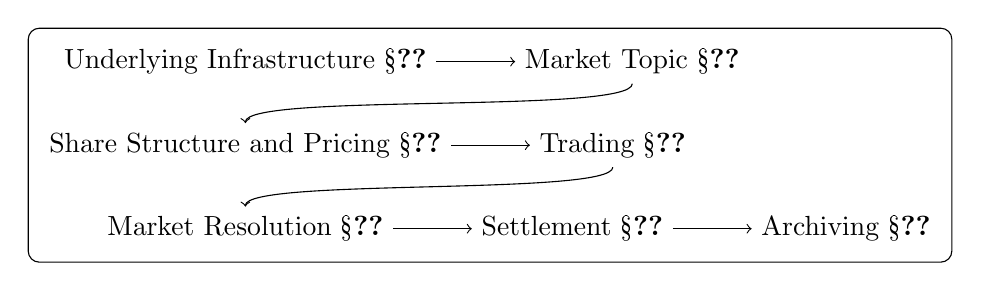
\begin{tikzpicture}[
  node distance=0.5cm and 1cm,
  show background rectangle,
  background rectangle/.style={draw, rounded corners, inner sep=6pt}
]

% Top row
\node (infra) {Underlying Infrastructure~\S\ref{wf:chain}};
\node[right=of infra] (topic) {Market Topic~\S\ref{wf:topic}};

% Middle row
\node[below=of infra] (shares) {Share Structure and Pricing~\S\ref{wf:price}};
\node[right=of shares] (trading) {Trading~\S\ref{wf:trade}};

% Bottom row
\node[below=of shares] (resolve) {Market Resolution~\S\ref{wf:close}};
\node[right=of resolve] (settle) {Settlement~\S\ref{wf:clear}};
\node[right=of settle] (archive) {Archiving~\S\ref{wf:archive}};

% Arrows
\draw[->] (infra) -- (topic);
\draw[->] (topic) to[out=-90, in=90, looseness=0.2]  (shares.north);
\draw[->] (shares) -- (trading);
\draw[->] (trading) to[out=-90, in=90, looseness=0.2]  (resolve);
\draw[->] (resolve) -- (settle);
\draw[->] (settle) -- (archive);

\end{tikzpicture}
}
\end{center}


We now turn to the design landscape of \depms and step through our modular workflow (\cf~\cite{ClEsGS21}), summarized above. Some design decisions will be common issues for both centralized and decentralized prediction markets. We include these anyways for completeness. However we put the emphasis on discussing design decisions that are pertinent to decentralization and permissionlessness.

% = = = = = = = = = = = = = = = = = = = = = = = = = = = = = = = = = = = = = = = = = = = = = = = = 

\subsection{Underlying Infrastructure}
\label{subsec:blockchain_infra}\label{wf:chain}

In theory, a decentralized and permissionless system might run on something other than a blockchain, but blockchain technology underlays all known \depms. The earliest (pre-Ethereum) research was in agreement that Bitcoin Script was not powerful enough to operate a \depm, and a \textit{sidechain}~\cite{BCD+14} would be required~\cite{Sz14,BCFKMN14}. Today, projects tend to run as \textit{smart contracts} on an Ethereum competitor (\eg Polygon~\cite{AKN21} or Solana~\cite{Yak18}) or an Ethereum L2 (\eg Arbitrum~\cite{KGCWF18} or Optimism~\cite{op}). There are no strong qualitative differences between the underlying blockchain---it is a choice driven by fees, user base, and supporting infrastructure. One other approach (\eg Zeitgeist~\cite{zeit} or SX Network~\cite{sx}) is to put the prediction market logic into the blockchain rules themselves on a custom \textit{app-chain}.

%MEV?

%Non-blockchain

% = = = = = = = = = = = = = = = = = = = = = = = = = = = = = = = = = = = = = = = = = = = = = = = = 

\subsection{Market Topic}\label{wf:topic}

% !TEX root = ../main.tex

% = = =

\begin{table}[t!]

\caption{Some pitfalls that illustrate the difficulty in properly defining a prediction market topic. \label{tab:pitfalls}}

\begin{tabular}{L{0.2\textwidth} L{0.8\textwidth}}
\hline
\textbf{Pitfall} & \textbf{Description} \\
\hline

% = = =

\multirow{2}{\linewidth}{Borderline Categories}
  & \textit{Example}: A market on whether Zelensky would wear a suit was contested when he wore a single-breasted jacket with patch chest pockets and matching trousers;\tablefootnote{\polyurl{Will Zelenskyy wear a suit before July?}{https://polymarket.com/event/will-zelenskyy-wear-a-suit-before-july}} media equivocated on describing it as a suit.\tablefootnote{Google Docs: \href{https://docs.google.com/document/d/1p0CSpse6YwLApvwKt173bDg1cQVNcNEe0_2sNCvhaZs/}{Did President Zelenskyy wear a suit before July 2025?}.} \\ \cline{2-2}
  & \textit{Mitigation}: Clearly state inclusion/exclusion criteria (\eg a subsequent market on a potential hug between Trump and Putin spent a paragraph defining a hug.\tablefootnote{\polyurl{Will Trump and Putin hug on Friday?}{https://polymarket.com/event/will-donald-trump-and-vladimir-putin-hug-on-friday}}) \\ \hline
  
  % = = =

\multirow{2}{\linewidth}{Precedence Gaps}
  & \textit{Example}: A proposition bet on the colour of the 2014 Super Bowl  `Gatorade shower' was contested when the coach was showered twice with different colours~\cite{BCFKMN14}. A market on whether Zelensky would be `the' 2022 TIME Person of the Year was contested when both Zelensky and the Spirit of Ukraine were named.\tablefootnote{\polyurl{Will Volodymyr Zelenskyy be the 2022 TIME Person of the Year?}{https://polymarket.com/event/will-volodymyr-zelenskyy-be-the-2022-time-person-of-the-year}} \\ \cline{2-2}
  & \textit{Mitigation}: Parse the predicate for any statements needing explicit precedence (\eg first, majority, primary); or establish a payout rule for ties; or include an outcome for `multiple.' \\ \hline

% = = =

\multirow{2}{\linewidth}{Hidden Presumptions}
  & \textit{Example}: A market concerning a divorce presumes the couple are married (as opposed to common law) which was unknown.\tablefootnote{\polyurl{Astronomer Divorce Parlay}{https://polymarket.com/event/astronomer-divorce-parlay}} \\ \cline{2-2}
  & \textit{Mitigation}: Parse the predicate for any presumptive statements and remove/address them.\\ \hline

% = = =

\multirow{2}{\linewidth}{No Ground Truth}
  & \textit{Example}: A market on whether a US strike destroyed an Iranian nuclear facility was contested when each country reported different outcomes and no neutral third party was granted access to the site.\tablefootnote{\polyurl{Fordow nuclear facility destroyed before July?}{https://polymarket.com/event/fordow-nuclear-facility-destroyed-before-july}} A market on whether Baron Trump was `involved' in the \$DJT memecoin lacked an authoritative source.\tablefootnote{\polyurl{Was Barron involved in \$DJT?}{https://polymarket.com/event/was-barron-involved-in-djt}} An election market on Venezuela's president was contested when the government declared Maduro won, while international media and democracy watchdogs declared Gonzalez received more votes.\tablefootnote{\polyurl{Venezuela Presidential Election Winner}{https://polymarket.com/event/venezuela-election-winner}} \\ \cline{2-2}
  & \textit{Mitigation}: Avoid markets without ground truth sources; or include an additional option in the market for unverified. \\ \hline

% = = =

\multirow{2}{\linewidth}{Platform Coupling}
  & \textit{Example}: Hypothetically, traders who correctly predict USDC will completely de-peg on a platform that pays out in USDC will receive a payout but it will be worthless (\cf~\cite{BCFKMN14}). \\ \cline{2-2}
  & \textit{Mitigation}: Avoid markets that are self-referential, including topics on the platform itself and its numinaire. \\ \hline

% = = =

\end{tabular}
\end{table}

% = = =

\cepms include the Iowa Electronic Markets~\cite{iem}, Kalshi~\cite{kalshi_docs}, and PredictIt~\cite{predictit_faq}, as well as InTrade historically~\cite{intrade}. These systems exercise control over what topics may form a market and thus are \textit{permissioned} with respect to market topics. They also operate under regulations that may restrict markets to certain topics or fully ban operations in regulated jurisdictions~\cite{Du19,Ma24}. 

By contrast, \depms like Augur~\cite{AKPWZ15,AKPWZ19}, the original Gnosis~\cite{Gn17}, and PlotX~\cite{plotx_docs} enable \textit{permissionless} market creation by any user without centralized review. This removes the regulatory hook, enables niche topics that might not attract mainstream interest~\cite{WZ24}, and allows markets to be created without delay after real world events. However it can also lead to a greater incidence of malformed (or even malicious) market definitions, spam duplicates of existing markets, and unlawful topics, such as the `assassination markets' which appeared on Augur in 2018~\cite{Du19}. \depms are generally web3 applications which means that a web-based user interface mediates transactions between the user and the underlying smart contracts. Market topic moderation could be implemented at the web3 layer (\eg Predictions.Global unlisted assignations markets from Augur's smart contracts~\cite{Du19}) but this does not prevent users from building an alternative UI or directly transacting with the smart contracts. 

%While \depms have the option to operate permissionlessly, they may also choose to permission market creation while leaving other aspects permissionless. At the time of writing, Polymarket is considered a \depm and while market topics can be suggested by users, final approval is made by a Market Integrity Committee.

These systems are not all purely permissionless. A \textit{hybrid model} puts some controls on topic creation without centralizing it fully~\cite{AKPWZ19}. For example, proposers may have to stake tokens to propose a market, and while the market is optimistically published, a review (either centralized or via an on-chain voting mechanism) could remove the market and/or slash the proposer.  

Careful attention must be paid to both the general topic of the market and the `fine-print' or exact predicate that decides the market. Table~\ref{tab:pitfalls} provides several examples of pitfalls. Dealing with definitional pitfalls has been, to date, a trial and error process where market creators learn from past mistakes and ad hoc `legalese' (e.g., a `consensus of credible reporting' may be used to resolve markets) is copied from market to market~\cite{Ad24}. Future research could develop machine-checkable predicate specifications (precedence rules, ranked sources, time semantics, and default outcomes) and verify they are well-defined with model checking (\cf~\cite{Cla21}). 

If issues in a market's topic or definition are uncovered while the market is still active, \depms like Polymarket allow `additional context' notes to be added. However these clarifications could alter the market ex post and also disadvantage traders who do not see the note. The latter can be mitigated by advertising that a note will be published, always publishing at the same time (\eg 5pm ET), and clearing standing limit orders from an orderbook before posting~\cite{poly}.

% = = = = = = = = = = = = = = = = = = = = = = = = = = = = = = = = = = = = = = = = = = = = = = = = 

\subsection{Share Structure and Pricing}\label{wf:mech}\label{wf:price}

The core requirement of a prediction market is that wagers are represented by fungible outcome shares. The structure of outcome shares typically falls into one of three categories and two variants (although more exotic structures are possible and explored in research). 

\subsubsection{WTA.}

The first structure we term \textit{winner-take-all (WTA)} (\aka \textit{categorical}) and was popularized by Iowa Electronic Markets~\cite{iem}. Consider a market with three possible outcomes: $\Omega=\{\mathsf{A}, \mathsf{B}, \mathsf{C}\}$.  A WTA market issues an outcome share for each outcome $J=\{j_\mathsf{A}, j_\mathsf{B}, j_\mathsf{C}\}$. If there are only two outcomes, it is called a \textit{binary market}. If the outcome $\omega$ is $\mathsf{B}$, the share $j_\mathsf{B}$ pays \$1 (or one unit of numeraire $\mathcal{N}$) and the other shares pay \$0.  For any $k\in\{\mathsf{A},\mathsf{B},\mathsf{C}\}$,

\begin{equation}
R_{j_{\mathsf{k}}}(\omega)=\begin{cases}1, & \text{if } \omega=\mathsf{k},\\0, & \text{otherwise.}\end{cases}
\end{equation}

For a WTA market to be well-functioning, two conditions must hold on outcome shares. (i) They should be \textit{mutually exclusive} so no more than one share wins: $R_{j_{\mathsf{k}}}(\omega)R_{j_{\mathsf{\ell}}}(\omega)=0 \quad \forall\omega\in\Omega, \forall\mathsf{k}\neq\mathsf{\ell} $; and (ii) they should be \textit{complete} so at least one share wins: $\sum_{\mathsf{k}\in\Omega} R_{j_{\mathsf{k}}}(\omega)=1\quad \forall \omega\in\Omega$. If they are not mutually exclusive, the operator could be under-collateralized for making all payments (in violation of solvency in Definition~\ref{def:axioms}). If they are incomplete, a deficient market might end with all participants receiving \$0. A consequence is that holding one share for each outcome is equivalent to holding \$1, a fact we will return to in \S\ref{wf:trade}. 

In a WTA market, the price of a outcome share (\eg $p(j_\mathsf{A})=\$0.54$) is a proxy for the probability that the outcome will occur (\eg $\mathrm{Pr}[\omega=\mathsf{A}]=54\%$). A common adage is the prices of each share sum to \$1.00 ignoring fees and discounting (\eg $p(j_\mathsf{A})=\$0.54$, $p(j_\mathsf{B})=\$0.23$, $p(j_\mathsf{C})=\$0.23$) but this is imprecise~\cite{BCFKMN14}. Outcome shares (like anything) have two prices: a bid price (what a trader is willing to buy for) and an ask price (willing to sell for). If the sum of the bid prices exceeds \$1.00 or if the sum of ask prices are below \$1.00, arbitrageurs have an opportunity to secure risk-free profit through a trade that will erase the condition when fully extracted. This means the sum of bids and sum of asks should result in the bid-ask spread straddling \$1.00 but the amount of the spread could be arbitrarily large. So in user interfaces that display a single `price' (\eg the last sale price or the midpoint between the best bid and the best ask), prices may indeed not sum to \$1.00---this is not a market failure, just a misunderstanding.  

 % = = =
 
 \subsubsection{YNB.}
 
The second structure we term a \textit{yes-no bundle (YNB)}. YNB markets were popularized by InTrade~\cite{intrade}. A YNB market issues two outcome shares for each outcome, a `yes' and a `no:'  $J=\{j_{\mathsf{A_Y}}, j_{\mathsf{A_N}}, j_{\mathsf{B_Y}}, j_{\mathsf{B_N}}, j_{\mathsf{C_Y}},j_{\mathsf{C_N}} \}$. For any $k\in\{\mathsf{A},\mathsf{B},\mathsf{C}\}$,

\begin{equation}
R_{j_{\mathsf{k_Y}}}(\omega)=
\begin{cases}
1, & \text{if } \omega=\mathsf{k},\\
0, & \text{otherwise.}
\end{cases}
\qquad
R_{j_{\mathsf{k_N}}}(\omega)=
\begin{cases}
1, & \text{if } \omega\neq\mathsf{k},\\
0, & \text{otherwise.}
\end{cases}
\end{equation}

Each outcome-specific pair $\{j_{\mathsf{k_Y}}, j_{\mathsf{k_N}}\}$ constitutes a binary WTA market ($\mathsf{k}$ vs.\ not-$\mathsf{k}$). A YNB market is the union of these pairs, so the WTA exclusivity and completeness properties hold per pair. However exclusivity and completeness do not necessarily hold across all bundles, allowing more flexible markets. For example, a market on what words Trump will say in a congressional address included Bitcoin (no), beautiful at least 10 times (yes), and Canada (yes).\footnote{\polyurl{What will Trump say during address to Congress?}{https://polymarket.com/event/what-will-trump-say-during-state-of-the-union?tid=1755462445353}} Multiple words can resolve to yes (not exclusive) and it is possible he says none of the listed words (not complete). An established YNB market that is being actively traded, because it is not complete, can have new outcomes added to it fairly, whereas WTA markets must account for every possible outcome at the start of the market (perhaps utilizing an `other' outcome).

\subsubsection{YNB-NR.}

A variant of the YNB market is one where, even though it is not necessary, the yes share outcomes are in fact complete and exclusive. In other words, each yes/no bundle is a WTA market and the set of all yes shares is also a WTA market. We term this YNB variant as \textit{negative risk} (YNB-NR), a term introduced by Polymarket~\cite{poly}. Recall that in a WTA market, roughly speaking, the share prices sum to \$1 (modulo the fine print about bid/ask spreads above). For a YNB-NR market, the Yes shares sum to \$1, while the No shares will sum to $|\Omega|-1$. 

The HBO documentary market from Section~\ref{sec:hbo} is an example of a YNB-NR market (Polymarket markets are either YNB or YNB-NR\footnote{Dune Analytics: `\href{https://dune.com/filarm/polymarket-activity}{Polymarket - Activity and Volume}' compares YNB (called CTF there) and YNB-NR (called negrisk there) statistics.}). This market was intended to be exclusive and complete across bundles by including a bundle for the outcome: `other/multiple.' Holding a No outcome share for Hal Finney has the same payoff as holding a Yes share for every other candidate. Polymarket introduced a \textit{negRisk} gadget that allows a trader to convert any No share into a portfolio of Yes shares for every other outcome. This enables traders to adjust their positions with less buying/selling on the markets, and also aligns prices between Yes and No markets with low friction arbitrage opportunities. Formally, a single No share has the equivalence (\ie same payoff ignoring fees and discounting):

\begin{equation}
j_{\mathsf{k_N}} \equiv \sum_{\ell \in \Omega\setminus\{\mathsf{k}\}} j_{\mathsf{\ell_Y}} \quad\text{for any }\mathsf{k}\in\Omega.
\end{equation}

And multiple No outcome shares can be converted into Yes shares plus cash:

\begin{equation}
\sum_{\ell \in \Omega\setminus\{\mathsf{k}\}} j_{\mathsf{\ell_N}}
\equiv
j_{\mathsf{k_Y}} + \$1\cdot(|\Omega|-2)
\end{equation}



% = = = 

\subsubsection{Scalar.}

The third structure is a market where the outcome is a quantity of interest (\eg popular vote, temperature, price level, \etc) observed at a cutoff time with a strict lower bound and upper bound. Termed a \textit{linear} or \textit{scalar} market, there is only one share and its payout is what value the quantity takes on (typically normalized to the range $[0,1]$ with rounding). As an example, in a market on Trump's popular vote, if the quantity is 49.8\%, the share will pay \$0.498. Shares can also be sold in bundles with `long' receiving \$0.498 and `short' receiving (\$1-\$0.498).

Formally, if we let $X:\Omega\to\mathbb{R}$ be the observed quantity, and $[a,b]$ be an interval of values, then the linear outcome share $j_{\mathrm{lin}}$ pays:

\begin{equation}
R_{j_{\mathrm{lin}}}(\omega)=
\begin{cases}
0, & X(\omega)\le a,\\
\dfrac{X(\omega)-a}{\,b-a\,}, & a< X(\omega) < b,\\
1, & X(\omega)\ge b.
\end{cases}
\end{equation}


While scalar markets are supported by \depms like Augur~\cite{AKPWZ15,AKPWZ19} or those based on Gnosis' Conditional Tokens Framework (CTF)~\cite{ctf}, including Polymarket~\cite{poly} and Omen~\cite{Omen_docs}, they are not frequently used. For Polymarket, markets instead cheat, approximating a scalar market  by splitting the quantity into `buckets' and running a YNB market for each bucket. This avoids a less-vetted codebase within CTF, unifies the user interface across market types, and possibly avoids small edge cases over the exact resolution of the quantity (\eg off by 0.1 percentage disputes). However a problem with buckets is as follows: Alice estimates correctly that Trump will win the election with 49--51\% of the popular vote. If there is a bucket for 45--49.9\% and a bucket for 50--54.9\%, Alice's forecast does not fit into a single bucket. Alice buys both buckets, knowing only one will win, diluting her expected return on capital. A second consequence of bucketization is volatile market jumps when the market consensus crosses from one expected bucket into a neighbouring bucket.\footnote{\polyurl{April 2025 Temperature Increase (ºC)}{https://polymarket.com/event/april-2025-temperature-increase-c4}} 

% = = = = = = = = = = = = = = = = = = = = = = = = = = = = = = = = = = = = = = = = = = = = = = = = 

\subsection{Trading}\label{wf:trade}
% JC

A near universal difference between any \cepm and \depm is that a \depm allows outcome shares to be withdrawn from the platform, typically in a form compliant with a token standard such as ERC-20 or the more efficient ERC-1155~\cite{LDBR24}. Withdrawing outcome shares allows traders to exchange tokens outside of the platform and to compose with third party DeFi services, including on-chain trading, lending, and leverage~\cite{WPG+22}. Options for trading outcome shares can be broken into two steps: (i) how does the first outcome share come into existence and how does the first trader trade, and (ii) how do traders trade once a market has been established? 

\subsubsection{The first trade.} Probably the greatest evolution in \depms, from Truthcoin to Polymarket, concerns how the first trade happens. There are three options: \textit{automated bookmaking}, \textit{splitting}, and \textit{matching}. 

\textit{Automated bookmaking} was popularized through the academic work of Robin Hanson~\cite{Ha03,Han07b}, researched for Intrade~\cite{McC08}, and first suggested for \depms by Truthcoin~\cite{Sz14}, which heavily influenced Augur v1~\cite{AKPWZ15}. In this model, the operator sets initial prices for each outcome share (equivalent to setting market odds) and collateralizes enough payout money to cover a worst-case loss in its treasury (preserving solvency in Definition~\ref{def:axioms}). If Alice is the first trader, she can immediately trade with the operator. The operator is autonomous and sets buy/sell prices algorithmically, originally using Hanson's logarithmic market scoring rule (LMSR)~\cite{Han07b}. The key point is that the operator is Alice's counterparty; if Alice wins, the operator loses, and vice-versa. The pros are instant liquidity for the first trader and the cons are the risk to the operator of losing money and the burden of needing to set initial odds (getting them wrong increases the chances it loses). 

Acute readers might wonder the relationship between automated bookmaking and  an automated market makers (\eg Uniswap) discussed below. Roughly speaking, a WTA market run by automated bookmaking is termed a cost-function prediction market (CFPM) and a CFPM is equivalent in pricing (and trade costs) to an AMM (defined by a set of axioms) with the right invariant~\cite{FPW23}.

The second approach, \textit{splitting}, was first suggested for \depms by the Princeton \depm~\cite{BCFKMN14} based on the Iowa Electronic Market~\cite{iem}. Augur switched from automated book making to splitting in v2~\cite{AKPWZ19}, Gnosis implemented splitting in CTF~\cite{ctf}, and \depms built on CTF, including Polymarket~\cite{poly} and Omen~\cite{Omen_docs}, use it.

Recall that in a WTA market, exactly one share in a set of shares will payout \$1. This means that holding a complete portfolio of every share is equivalent (in payoff, ignoring fees and discounting) to holding \$1. A splitting gadget allows a trader to input \$1 and receive a portfolio contain 1 share of each outcome. Generally, a \textit{merging} gadget is also available where a complete set can be redeemed for \$1 at any time before the market closes. Alice can obtain a set of shares and list asking prices (through a limit order book or by being the first liquidity provider in an AMM) for some or all of the shares, and if Bob is willing to buy a share from Alice, the first trade occurs. The pros to splitting is that the operator has zero exposure to the market, while the con is that Alice must wait for a second trader, Bob, before she can trade. 

In YNB markets, each outcome’s YES/NO pair is its own two-outcome WTA market. Splitting is per outcome: converting \$1 of collateral mints one $j_{\mathsf{k_Y}}$ and one $j_{\mathsf{k_N}}$ for the chosen $\mathsf{k}$. Across outcomes, supplies are uncoupled---the total minted for the $\mathsf{A}$ bundle need not match that for $\mathsf{B}$ or $\mathsf{C}$. 

The third approach, \textit{matching}, was used by InTrade~\cite{intrade} and a variant by Fairlay~\cite{fairlay}. Briefly, it mirrors a futures market, where Alice posts a desired short/long position at a chosen price on an orderbook with a margin account holding enough cash to cover her maximum loss if she obtains the position. If Bob is willing to take the other side, also with sufficient margin for his maximum loss, the operator matches them, creates two shares and gives them to Alice and Bob. Alice and Bob are not counterparties, both settle with the operator once the shares are created, however their coincidence of wants (COW) is necessary for the operator to create shares at no risk to itself. Matching is operationally more complex and effectively requires a central limit order book or batch auction, which excludes is too expensive to run on-chain~\cite{MoCl23}. 


\subsubsection{Trading in established markets.}

Once outcome shares are in circulation, they can be traded any way fungible blockchain tokens can be traded. This includes \textit{centralized exchanges} that custody the tokens and use central order book (CLOBs); \textit{partially decentralized exchanges} where CLOB matching is done off-chain and settlement is done on-chain; or \textit{fully on-chain exchanges}, of which automated market makers (AMMs) are the most common. 

Of interest, AMMs were born out of Gnosis' research into automated bookmarking for prediction markets. They first developed alternatives to the LMSR rule, including the constant product rule~\cite{LK17}. In parallel, Bancor worked on exchanges where multiple traders could contribute tokens to a common liquidity pool. Uniswap v1 merged these two ideas to create the basic template of an AMM that is common today.

Circling back to automated bookmaking, splitting can be used in conjunction with AMMs to realize automated booking, as first used in Gnosis' closed beta Sight~\cite{Bar19}. An operator begins with $2n$ units of the numeraire, \eg $2n$ USDC. It takes half of the money, $n$ USDC, and uses the splitting gadget to obtain $n$ shares in each outcome. For each outcome share, it estimates the outcome probability as $p_i$ and starts an AMM with initial liquidity of $n$ outcome shares and $p_i\cdot n$ USDC. It repeats for each outcome. Thus assuming the probabilities sum to 1, the operator has split its remaining $n$ USDC across the AMMs. The operator can lose up to $2n$ USDC in divergence loss, assuming traders can split as well (and thus create the shares necessary to drain the AMM of its USDC), in addition to failing (through stale prices) to realize profits (\ie LVR~\cite{MMRZ22}). The important point is that the operator is still solvent per Definition~\ref{def:axioms} as the $2n$ USDC is either locked in the splitting gadget or locked in the AMM.

Despite the direct lineage between prediction markets and AMMs, AMMs are problematic for prediction market trading. \depm outcome shares behave in specific ways that differ from typical crypto-assets and tokens. The price is strictly bounded between \$0 and \$1, the value of a share can jump to \$0 or \$1 near-instantly when an event outcome is finalized, and once finalized, the price is permanent. When real world events occur, AMMs can be drained faster than liquidity providers can withdraw liquidity. Adapting AMMs to these constraints is an interesting open problem. Paradigm’s pm-AMM tapers liquidity as a scheduled expiry approaches, which helps for events that crystallize over a fixed time horizon~\cite{MR24}; but many markets jump or resolve unexpectedly, falling outside of the model used for the results.

When trading on-chain, miners and other users can front-run transactions, an area of study called maximum extracted value (MEV)~\cite{BBDGJKLZ19}. Although the term MEV did not exist at the time, the Princeton \depm describes the MEV problem extensively~\cite{BCFKMN14} and proposes a mitigation now called a frequent batch auction (FBA) (again, the term FBA was not popularized until later~\cite{BCS15}).

A final trading-relevant subject for prediction markets is arbitrage. Arbitrageurs ensure market prices are consistent, for example across all shares in a WTA market or between Yes/No bundles in a YNB market. A recent paper studies combinatorial arbitrage on Polymarket between markets with logically related predicates (\eg Republicans win the presidency; Trump wins the presidency) and measures roughly \$40M USD of realized arbitrage profits over the measurement period~\cite{SGKS25}. 

%\textblue{Add cross \depm arbitrage as well. https://x.com/MovieTimeDev/status/1966515883355848889}

% = = = = = = = = = = = = = = = = = = = = = = = = = = = = = = = = = = = = = = = = = = = = = = = = 

\subsection{Market Resolution}\label{wf:close}

It is possible that a market topic can be determined on-chain (\eg total value locked in a DeFi service) in which case resolution is simple, however typically, prediction market outcomes concern facts that are off-chain. In these cases, resolution is the process of finalizing an off-chain outcome in an on-chain market. The predominate approaches are the following: self-settling markets, auto-resolve rules, using a designated arbiter, using a network of reporters, and crowdsourcing a vote. The term \textit{oracle} is commonly used for any of the latter three approaches (while the first two could be considered oracle-less). 

A \depm will probably use a \textit{hybrid} or \textit{chained approach} that does not rely on a single method. For example, an arbiter from an allowlist might be able to propose a market outcome while also allowing disputes from anyone. If an outcome is disputed, it is escalated to a crowdsourced vote. If the vote is considered defective, a further escalation could allow an Admin account to overrule the decision. The ultimate backstop is the law which would not stop a wrong outcome but could be used to remunerate parties damaged by it.

\subsubsection{Oracle-less approaches.}

A \textit{self-settling market} is based \textit{splitting} and \textit{merging} (see \S\ref{wf:trade}) of shares and relies on participants with winning shares to purchase the losing shares (for close to \$0) and redeem \$1 by merging them~\cite{BMR17}. If losing shares do not trade near \$0 or become illiquid, the broader market might accept winning shares as a substitute for dollars. If a market outcome is contentious with no recognized winner (\eg a poorly defined market in \S\ref{wf:topic}), the market will not settle. An \textit{auto-resolve rule} could also be used such that outcomes are finalized when, say, their token trades above \$0.99 for at least $t$ time. Auto-resolve rules are subject to market manipulation (losing shares are wash traded near \$1 long enough to finalize, in which case they are worth \$1) or griefing attacks (yes shares are traded below \$0.99 to prevent finalization). While an auto-resolve rule is too fragile to rely on solely, it could be used optimistically to provide an initial settlement; only disputed cases would be escalated to an oracle~\cite{Aug15}. 

\subsubsection{Designated arbiters.}

Typically a \cepm will decide events within the platform~\cite{kalshi}. A \depm might outsource decisions to a trusted organization, such as the Associate Press (AP) which experimented with writing US election results into Ethereum.\footnote{Etherscan: \url{https://etherscan.io/address/0x0792724900B551d200D954a5Ed709d9514d73A9F}} From a trust perspective, this is equivalent to using an AP \cepm, but from a logistics perspective, it is simpler to AP to be an oracle than to run an entire \cepm. Further, it allows \textit{trust agility} where AP can be replaced by a competing source with minimal disruption~\cite{BCFKMN14}. A \depm might also used a designated party only as a last resort if other methods lead to a contentious result~\cite{Rey24}. 

Recently interest is in evaluating arbitration through an AI system~\cite{chaos}. A 2025 Chainlink study poses 1,660 Polymarket questions to LLMs and reports ~89.3\% accuracy (sports 99.7\%, politics 84.3\%)  with temporal-reasoning challenges~\cite{ZVW25}. AI can also be used in agent-mode, tasked with actively gathering evidence and reporting if resolution can be reached~\cite{chaos}. AI oracles are potentially vulnerable to adversarial manipulation and poisoning attacks~\cite{ZGWJ25}, and may recall incorrect facts that are incorrectly stated in the training data. An over-reliance on AI systems in generating news, trading in markets based on news, and settling markets based on news could result in bad interactions or negative feedback loops. 

\subsubsection{Reporter networks.}

Some oracle systems focus on quickly reporting on updating values~\cite{BCCJM21}, such as an asset price or a sports score which could naturally settle some types of prediction markets, such as rapid markets from Augur Turbo~\cite{aug25} and Polymarket~\cite{polylink}. Generally a set (or network) of arbiters (or reporters) will report the value and an aggregation method (\eg median value or a mean value after outlier filtering for quantitative data, mode for qualitative) will update the value on-chain~\cite{ClEsGS21}. Updates are emitted when deviation or heartbeat thresholds are met, giving explicit control over latency/recency and bounding staleness under network stress. A \depm can read the aggregator at a fixed resolution time and settle without discretionary intervention~\cite{aug25,thalesmarket_docs}. 








\subsubsection{Crowdsourced vote.}

A final mechanism is to determine off-chain facts by polling a set of willing participants~\cite{But13,Sz14,AKPWZ15,AKPWZ19,uma,kleros}. This procedure is defined by four design choices:

\begin{enumerate}
\item \textit{Electorate}: participants stake governance tokens to enrol and votes are either held with all participants, or with a randomly selected subset of all participants.
\item \textit{Ballots:} may be visible to other participants or may be hidden until voting closes (typically with a two-round commit-reveal protocol but more sophisticated methods could be used~\cite{GSZB23}).
\item \textit{Aggregation:} votes are weighed by the amount of staked tokens, categorical questions are decided by plurality (perhaps with minimum quorum) while quantities with a median or smoothed mean. 
\item \textit{Incentives:} participants who affirmed the final result in their individual votes receive rewards, while those who did not will at least forgo rewards, but might also have their participation tokens slashed. 
\end{enumerate}

The precise parameters of these systems vary significantly across many different designs, while deployed systems like UMA's data verification mechanism (DMV)~\cite{uma} and Kleros~\cite{kleros} have settled billions of dollars. Topics like fee mechanisms and proof of stake consensus protocols have received much academic attention, but incentive-compatible designs and formal proofs for oracles is largely under-explored. By contrast, a growing theoretical line proposes truth-elicitation schemes with formal guarantees~\cite{Pre04,SKC25}. However in practice, uptake is absent, in part because these designs are complex to run, sensitive to Sybil attacks, and can fail if voters rely on a common source of information.

Token votes for \depms are hostile environments where an attacker’s external payoff from a wrong resolution exceeds the system’s economic security, which can lead to failure~\cite{FoBo19}. Rational voters are incentivized to agree with the majority, rather than necessarily reporting the ground truth (a situation colloquially known among economists as a Keynesian beauty contest). The system often works because the ground truth is an obvious point where participants will coordinate (known as a Schelling point), however voters might fear voting for truth if large token holders (whales) visibly stake on a wrong outcome early in the vote. An example\footnote{\polyurl{Ukraine agrees to Trump mineral deal before April?}{https://polymarket.com/event/ukraine-agrees-to-give-trump-rare-earth-metals-before-april}} occurred on Polymarket~\cite{Rey25}, leading to concerns of token concentration within the UMA token. At the time of writing, the top five UMA wallets UMA control ~45.6\% of votes and the top 13 exceed 65\%, enough to meet the passing threshold.\footnote{Dune Analytics: \href{https://dune.com/uma\_protocol/uma-protocol}{\$UMA Voting Participation}} If successful attacks depress token prices, the attacks become cheaper, potentially creating a spiral (\cf~\cite{KM21}). 

These concerns affirm design decisions like a secret ballot, using subsets of participants in a vote (potentially split by subject expertise), and redrawing larger panels on appeal with higher bonds/fees to raise capture costs only when disputes persist.

% = = = = = = = = = = = = = = = = = = = = = = = = = = = = = = = = = = = = = = = = = = = = = = = = 

\subsection{Settlement}\label{wf:clear}

The slogan `sweat the game, not the payout~\cite{Fu24}' is used to differentiate regulated sportsbook operators from `neighbourhood bookies,' however even legitimate operators in the US have allegedly denied payouts using a legal loophole.\footnote{A law protects sports books from obvious errors, like a `fat finger' when setting odds, but can be misused to claim long-shot bets were `obvious mistakes' after the fact~\cite{Fu24}.} The advantage of a \depm in this context is two-fold: (i) payouts are fully (or largely) autonomous, not subject to human discretion, and (ii) the share structure ensures the operator has zero risk (or predetermined bounded risk, in the case of automated bookmaking) and is therefore financially indifferent to making any fair payout (see the solvency axiom in Definition~\ref{def:axioms}).


% Split payouts possible in Truthcoin: 0.5/0.5

Once the market is resolved, a \depm will enable each winning share to be converted into 1 unit of the numeraire (\eg 1 USD in a stablecoin) and transferred into the user's self-custody. While a \depm in theory could \textit{push} payouts to users, it is common to wait for the user to initiate the redemption---a \textit{pull} mechanism~\cite{ctf}. In this case, users pay the gas cost of the redemption which requires users to hold the native currency of the underlying blockchain. Polymarket offers gasless withdrawals (using OpenGSN relayers~\cite{gsn}), however users can bypass this at their choice. In a pull model, some users may not redeem their shares in a timely manner---a \depm may opt to sweep this surplus into its own capital or burn it, but \depms generally hold it on-chain in perpetuity. As with any smart contract allowing withdraws based account balances, hardening against reentrancy attacks is critical.


% = = = = = = = = = = = = = = = = = = = = = = = = = = = = = = = = = = = = = = = = = = = = = = = = 

\subsection{Archiving}\label{wf:archive}

Publicly accessible \depm data provides society with a useful forecasting tool, and archival datasets enable calibration, insight into historical events, and replication of findings. On-chain records (state, logs, and calldata) inherit strong archival and verification properties so long as the chain persists. These records can be replayed and exposed via deterministic chain indexers (\eg The Graph, SubQuery) or managed subgraph hosting (\eg Goldsky). Human-readable materials can be stored in content-addressed, peer-to-peer systems (\eg IPFS) and mirrored to permanence layers with economic durability (\eg Arweave, Filecoin), with their content identifiers anchored on-chain. Privately held operational data can be released as signed public snapshots or made queryable via open APIs.

Two kinds of artifacts matter most. First, the market semantics: the market topic, resolution rules, and any clarifications. Platforms such as Augur and Polymarket record stable on-chain identifiers (e.g., market/condition and token IDs) and keep the human-readable documents in content-addressed storage, with their content hashes/CIDs referenced on-chain. Second is the market data, including trading data (time, volume, price), outcome share supply and redemption totals, and timestamps for the status of the market (\eg opened, resolved, finalized). In practice, settlements and token movements are emitted on-chain, then replayed by deterministic chain indexers into queryable tables for research and UX. The same applies to the resolution process, its dispute trail and finalized outcome. If trading is off-chain (fully or partially), \depms will need to expose application indexes/APIs for fast access and publish signed public snapshots for reproducibility. This missing data includes detailed trading, order-book depth, and liquidity metrics.

For example, Polymarket settles markets on the canonical ledger using the UMA Optimistic Oracle (the dispute game) and writes the final payout vector into the Gnosis Conditional Tokens Framework (CTF) (the settlement contract); outcome shares are ERC-1155 tokens (a multi-token standard), so transfers, mints, and redemptions are visible in logs. Trades are matched off-chain on a central limit order book (CLOB) but settle on-chain, while detailed order-book depth, quotes, and liquidity metrics are exposed via Polymarket’s API (called Gamma). For reproducible research, the same on-chain events are also mirrored by deterministic chain indexers (subgraphs run by services such as Goldsky/The Graph), and API time series can be cross-checked against transaction hashes on the ledger.


% = = = = =

\section{Discussion and Research Agenda}

\paragraph{Composability.} Perhaps the biggest evolution in \depm design is infrastructure~\cite{Gun24}. Early \depms were monolithic, single-vendor codebases. Modern \depms are built from existing infrastructure, which composes through highly standardized interfaces. For example, Polymarket's core \depm code is Gnosis' conditional token framework~\cite{ctf}. The numeraire is Circle's USDC stablecoin, which can be bought with a credit card through MoonPay. Trading outcome shares and USDC works out-of-the-box on any platform (on- or off-chain) that supports ERC-1155 tokens. Market outcome disputes are escalated to UMA's DVM oracle~\cite{uma}. Polymarket also uses third party services for bridging assets, embedded wallets (based on email verification), and EIP-3009 gasless withdrawals. Beyond software engineering benefits, building a service by composing modules can enhance trust agility, which is the ability to quickly swap out modules that are faulty or malicious. For example, Polymarket could switch from UMA to say Chainlink or Kleros, with less effort than if the oracle service was vertically integrated. 

% !TEX root = ../main.tex

\begin{table}[t!]
\centering
\caption{DePM Design Decisions Across the Modular Workflow.}

\adjustbox{max width=\textwidth}{
\begin{tabular}{|l|c|c|c|c|c|c|c|c|c|c|}

\flatrow{Platform}  & \headrow{Infrastucture (\S\ref{wf:chain})} & \headrow{Permissionless Topic (\S\ref{wf:topic})} & \headrow{Share Structure (\S\ref{wf:price})} & \headrow{Numeraire  (\S\ref{wf:price})} & \headrow{Initial Issuance (\S\ref{wf:trade})} & \headrow{Permissionless Trading  (\S\ref{wf:trade})} & \headrow{Resolution  (\S\ref{wf:close})} & \headrow{Settlement  (\S\ref{wf:clear})} & \headrow{On-Chain Archiving  (\S\ref{wf:archive})} \\


\hline
Truthcoin~\cite{Sz14} & App-chain & \CIRCLE & Comb. & Pegged BTC & Auto Bookmaking &\CIRCLE & Token Vote & Pull & \CIRCLE \\
\hline
Princeton PM~\cite{BCFKMN14} & App-chain & \CIRCLE & WTA & Pegged BTC & Splitting & \CIRCLE & Designated Arbiter & Pull & \CIRCLE \\
\hline
Augur (v1)~\cite{AKPWZ15}  &  Smart Contract & \CIRCLE & WTA & ETH & Splitting &  \CIRCLE & Token Vote & Pull & \CIRCLE \\
\hline
Augur (v2)~\cite{AKPWZ19}  &  Smart Contract &\CIRCLE & WTA & DAI & Splitting & \LEFTcircle, \CIRCLE  & Token Vote & Pull & \LEFTcircle \\
\hline
Omen~\cite{Omen_docs}  &  Smart Contract & \LEFTcircle & CTF & DAI & Splitting & \CIRCLE & Designated Arbiter & Push & \LEFTcircle\\
\hline
Polymarket~\cite{poly}  & Sidechain & \Circle & YNB (-NR) & USDC & Splitting & \LEFTcircle, \CIRCLE & Optimistic, Token Vote & Pull* & \LEFTcircle \\
\hline
%PlotX (v2)~\cite{plotx_docs}  & Sidechain & \CIRCLE & B/S & CFMM & USDC & \Circle & Ext.O & PL & $\lozenge$ \\
%\hline
Zeitgeist~\cite{zeitgeist_docs} & App-chain & \LEFTcircle & WTA & Multi & Auto Bookmaking & \Circle & Designated Arbiter & Pull & \LEFTcircle \\
\hline
%Thales~\cite{thalesmarket_docs} & Smart Contract & \Circle & Binary & CFMM & Multi & \Circle & Ext.O & PL & $\blacklozenge$\\
%\hline
Kalshi~\cite{kalshi_docs} & Centralized  & \Circle & YNB & USD & Matching & \Circle & Designated Arbiter & Push & \Circle \\
\hline

\end{tabular}
}

\vspace{0.30em}
\begin{minipage}{\textwidth}
\textbf{Legend:} \\
%\textbf{Implementation:} \Circle = Paper only; \CIRCLE = System Implemented
%\textbf{Infrastructure:} Contract = Smart contract on Layer 1 or Layer 2; SideChain = Smart contract on sidechain (EVM altchain); AppChain= Custom Layer 1; DB = Database\\
%\textbf{Permissionless Topic:} \CIRCLE = Permissionless; \LEFTcircle = Supports permissionless framework; \Circle = Permissioned. Note: Thales uses a Sportsbook model, Kalshi uses a CFTC-compliant Rulebook, and Polymarket is piloting a hybrid approach with user-suggested topics.\\
%\textbf{Share Structure:} WTA = Winner-Take-All; CTF = Conditional Tokens; YNB-NR = Yes/No Bundle and Negative-Risk; Comb. = Combinatorial; B/S = Binary/Scalar; \\
%\textbf{Initial Issuance:} Split = complete-set minting; LSMR = Logarithmic Market Scoring Rule ; FPMM = fixed-product MM; CF: CFMM = constant-function MM; Matching = Matching CLOB \\
%\textbf{Numeraire:} CSH = CashCoin (1:1 redeemable to BTC); ZTG = Zeitgeist parachain native token; Multi = USDC, ETH, THALES \\
%\textbf{Trading:} \CIRCLE = decentralized CLOB (proposal only); DEX =  DEX (hybrid: off-chain matching + on-chain settlement); \Circle = AMM;  \\
%\textbf{Resolution:} REP = Augur REP; UMA = UMA optimistic; R/K = Realitio$\rightarrow$Kleros; VTC = VoteCoins; Ext.O = external oracle; C = centralized. \\
\CIRCLE, \LEFTcircle, \Circle respectively infer fully, partially or do not support the title of the column.\\
Keywords used in the table are fully defined in the related sections.\\
\textbf{Settlement:} * Polygon offers a gasless, meta-tx pull  \\
\end{minipage}
\end{table} 

\paragraph{Regulation.} In jurisdictions like the United States, both \cepms and \depms are tightly controlled and not always legal to operate~\cite{Du19,Ma24}. The paramount concerns of regulators are not specific to prediction markets or the difference in their microstructure from other forms of wagering (although market integrity is always a concern); rather, regulators control any kind of wagering on political events (a stance challenged by leading economists~\cite{AFGH+08}), as well as any kind of financial service offered to unaccredited consumers. For advocates of liberal markets, \depms are seen as a way to side-step regulation, particularly when the \depm is decentralized in most or all dimensions of our taxonomy. 


% Does polymarket need uma?
% Optimistic works - who has time ? 
% Discussion Points:
% Recursive markets (market topic is about another market)
% Insurance / hedging 
% Futurarchy
% Insider trading, asymmetric info, example: betting on software delays -> no surprises any more if PMs extract insider info and build it into prices
% Polymarket as news source (also circular feedback through LLMs, AI trained on market data, AI agents, AI generated news, AI oracles)

\paragraph{Research Agenda.}

The history of \depm shows a convergence toward trading outcome shares, creating by splitting, on CLOBs and AMMs. While many aspects of prediction markets have been studied formally, comparing different market microstructures has not received adequate research; and optimizing AMMs for \depms is still at the beginning stages~\cite{KS23,MR24}. Less convergence exists on how to decide market outcomes, a uniquely \depm problem (since a \cepm can arbitrate its own markets). Another way to look for research problems is to pinpoint where faulty behaviour is still occurring: for Polymarket, the biggest sources are poorly defined market topics and the vulnerability of market resolution to manipulation. Analysis of new approaches to either problem (formal verification for topics? AI as oracles?) would be welcome research, as would bringing a theoretical lens to deployed oracle voting systems to understand if formal guarantees about incentives can be made. A lesser known issue is archiving \depm data and developing tools that could fully `replay' a market at each timestep, which would be useful for understanding how markets incorporate news (real and fake) into prices. Finally, the degree to which \depms can be pushed further toward permissionlessness in all aspects is still largely open, particularly around setting topics for markets.

\section{Conclusion}

Researchers and builders have used a set of shifting designs, definitions, and vocabulary for \depms. We aim to provide a modular framework that is useful for careful comparison between systems with different design choices, showcasing the full set of choices available, uncovering unsolved research problems, understanding the history of \depm ideas, and providing a learning resource for those wanting to catch up on \depms. Our taxonomy does not identify a single best design but helps illustrate the trade-offs between them. 





% = = = = = Acknowledgements  =  =  =  =  = = %

\subsubsection*{Acknowledgements.} We thank the reviewers who helped to improve our paper. J. Clark acknowledges support for this research project from (i) the National Sciences and Engineering Research Council (NSERC), Raymond Chabot Grant Thornton, and Catallaxy Industrial Research Chair in Blockchain Technologies, (ii) the AMF (Autorité des Marchés Financiers), and (iii) NSERC through a Discovery Grant. 

% = = = = = Bibliography = = = = = %

\bibliography{bib/depm.bib}
%\nocite{*}

% = = = = = End Notes = = = = = %

\clearpage
\appendix
%% !TEX root = ../main.tex

\section{Modular Workflow}
 
The modular workflow for DPMs, detailed in sub-sections \ref{subsec:blockchain_infra} through \ref{subsec:economic_tradeoff} , outlines key components and decision pathways involved in platform development and operation. Initially, designers select an appropriate blockchain infrastructure, evaluating trade-offs between Layer-1 mainnet's decentralization and security versus Layer-2's cost and throughput efficiencies, considering bridging delays and associated security risks (Section~\ref{subsec:blockchain_infra}). Following this, market creation is structured by deciding on permissioned or permissionless market listing models (Section~\ref{subsec:market_setup_init}). Next, the workflow addresses the tokenization of market outcomes (Section~\ref{subsec:market_mechcanics}) and implements suitable trading mechanisms such as automated market makers (AMMs), limit order books, or a hybrid combination of both (Section~\ref{subsec:price_bootstrapping}). After market closure, the platform utilizes either centralized or decentralized oracle systems, including potential dispute resolution processes for contested outcomes (Section~\ref{subsec:market_resolution}). Subsequent stages involve selection of payout methods (automatic push or claim-based pull) and managing remaining funds or platform fees (Sections~\ref{subsec:payout_redemption}). The market metadata archival is preserved on-chain logs or decentralized storage services such as IPFS and Arweave (Section~\ref{subsec:archival}). Finally, economic trade-offs affect the popularity usability and adoption of the market ({Section~\ref{subsec:economic_tradeoff}). This modular workflow is visualized in Figure~\ref{fig:dpm_workflow} below.

\begin{wrapfigure}{rt}{0.4\textwidth}
    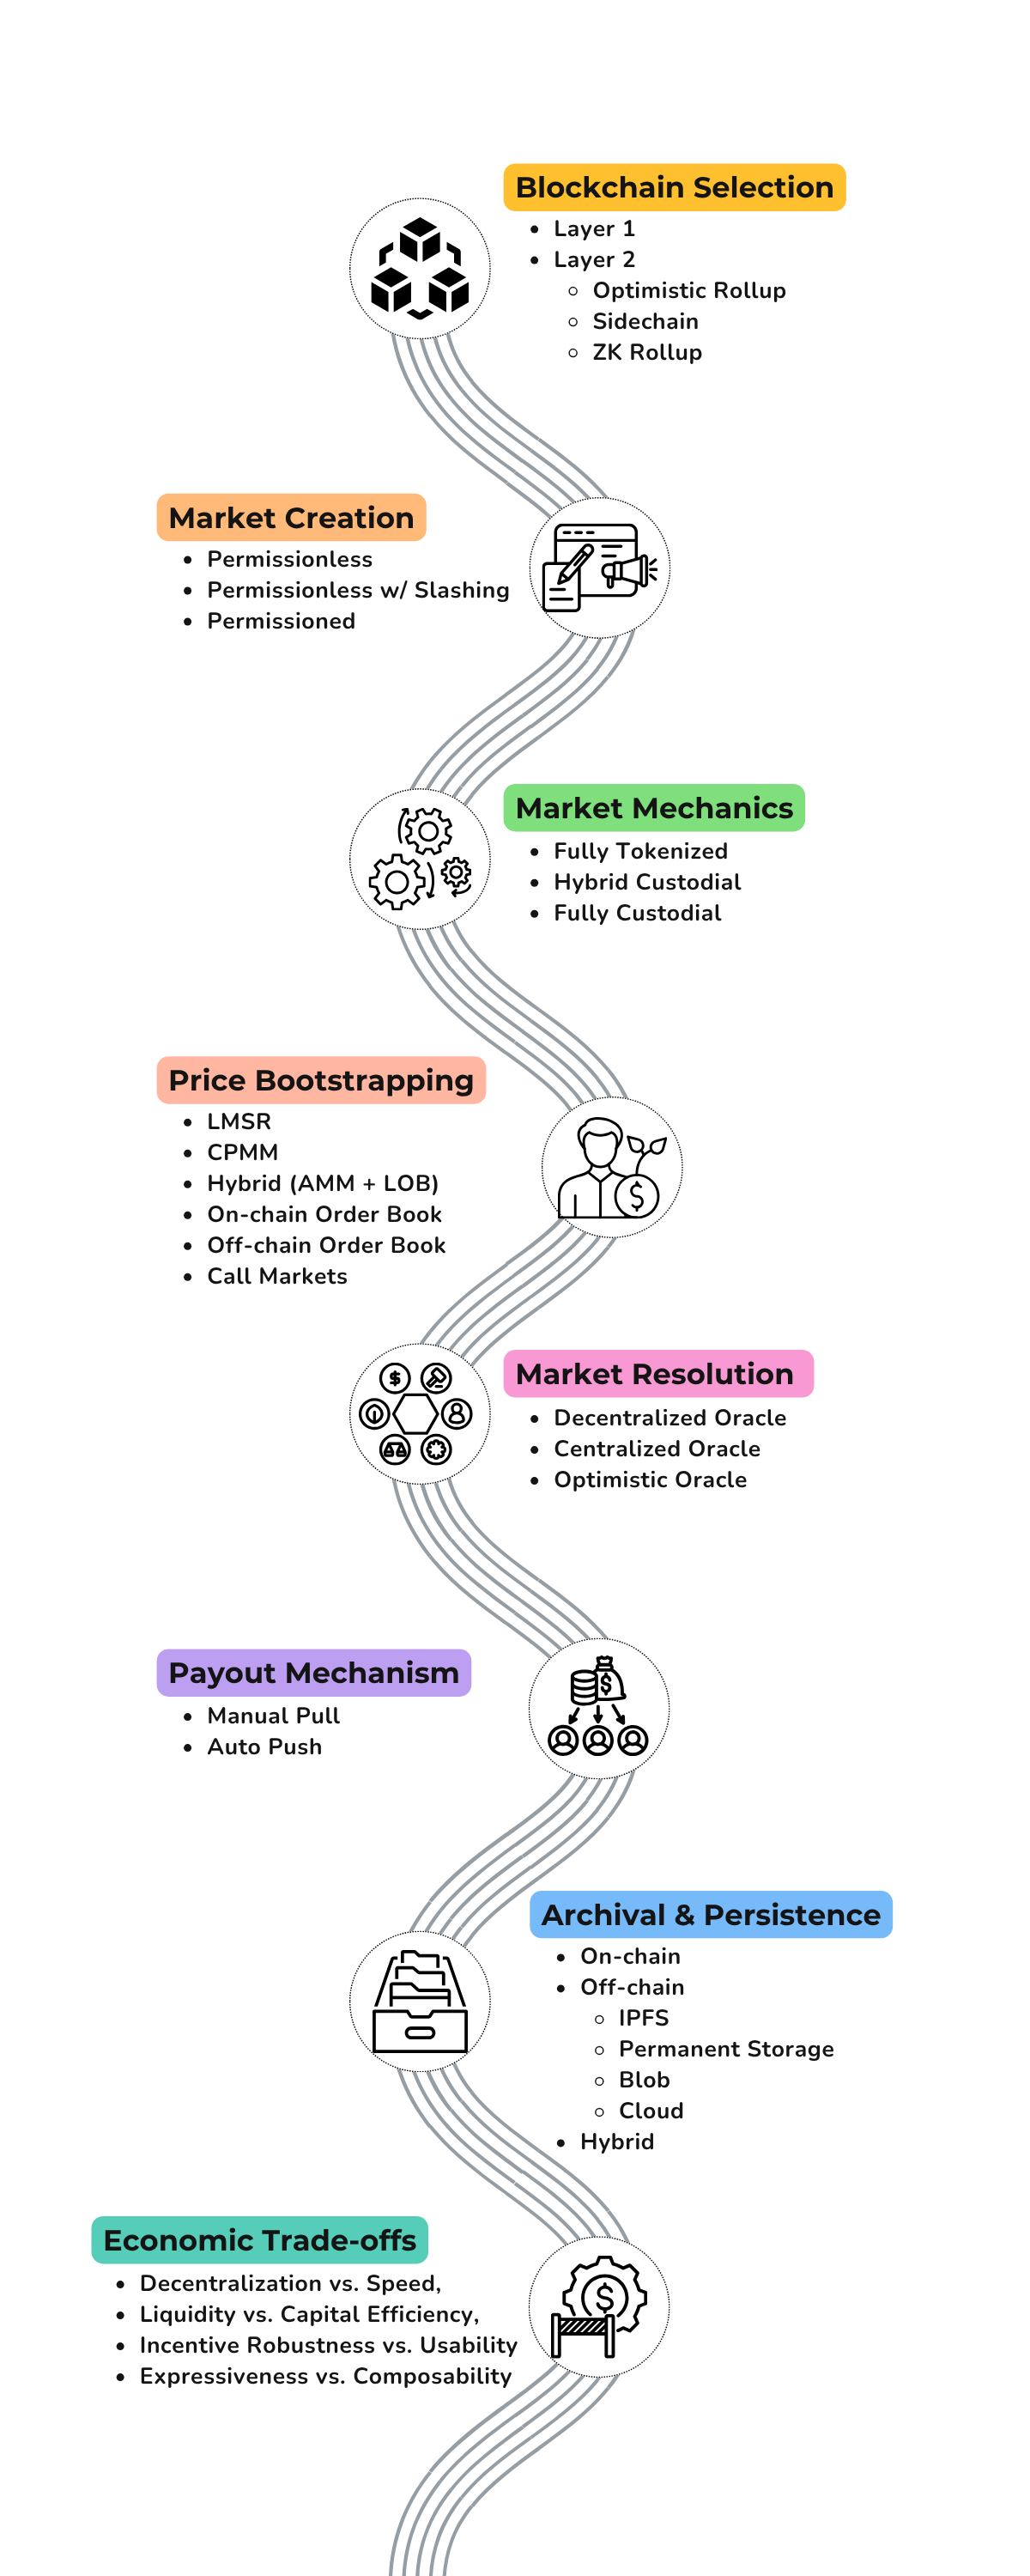
\includegraphics[height=0.75\textheight]{figures/fig_modular_workflow.png}
   \caption{Modular Workflow for Decentralized Prediction Market Platforms.}
    \label{fig:dpm_workflow}
\end{wrapfigure}

%\begin{figure}[htbp]
%    \centering
%    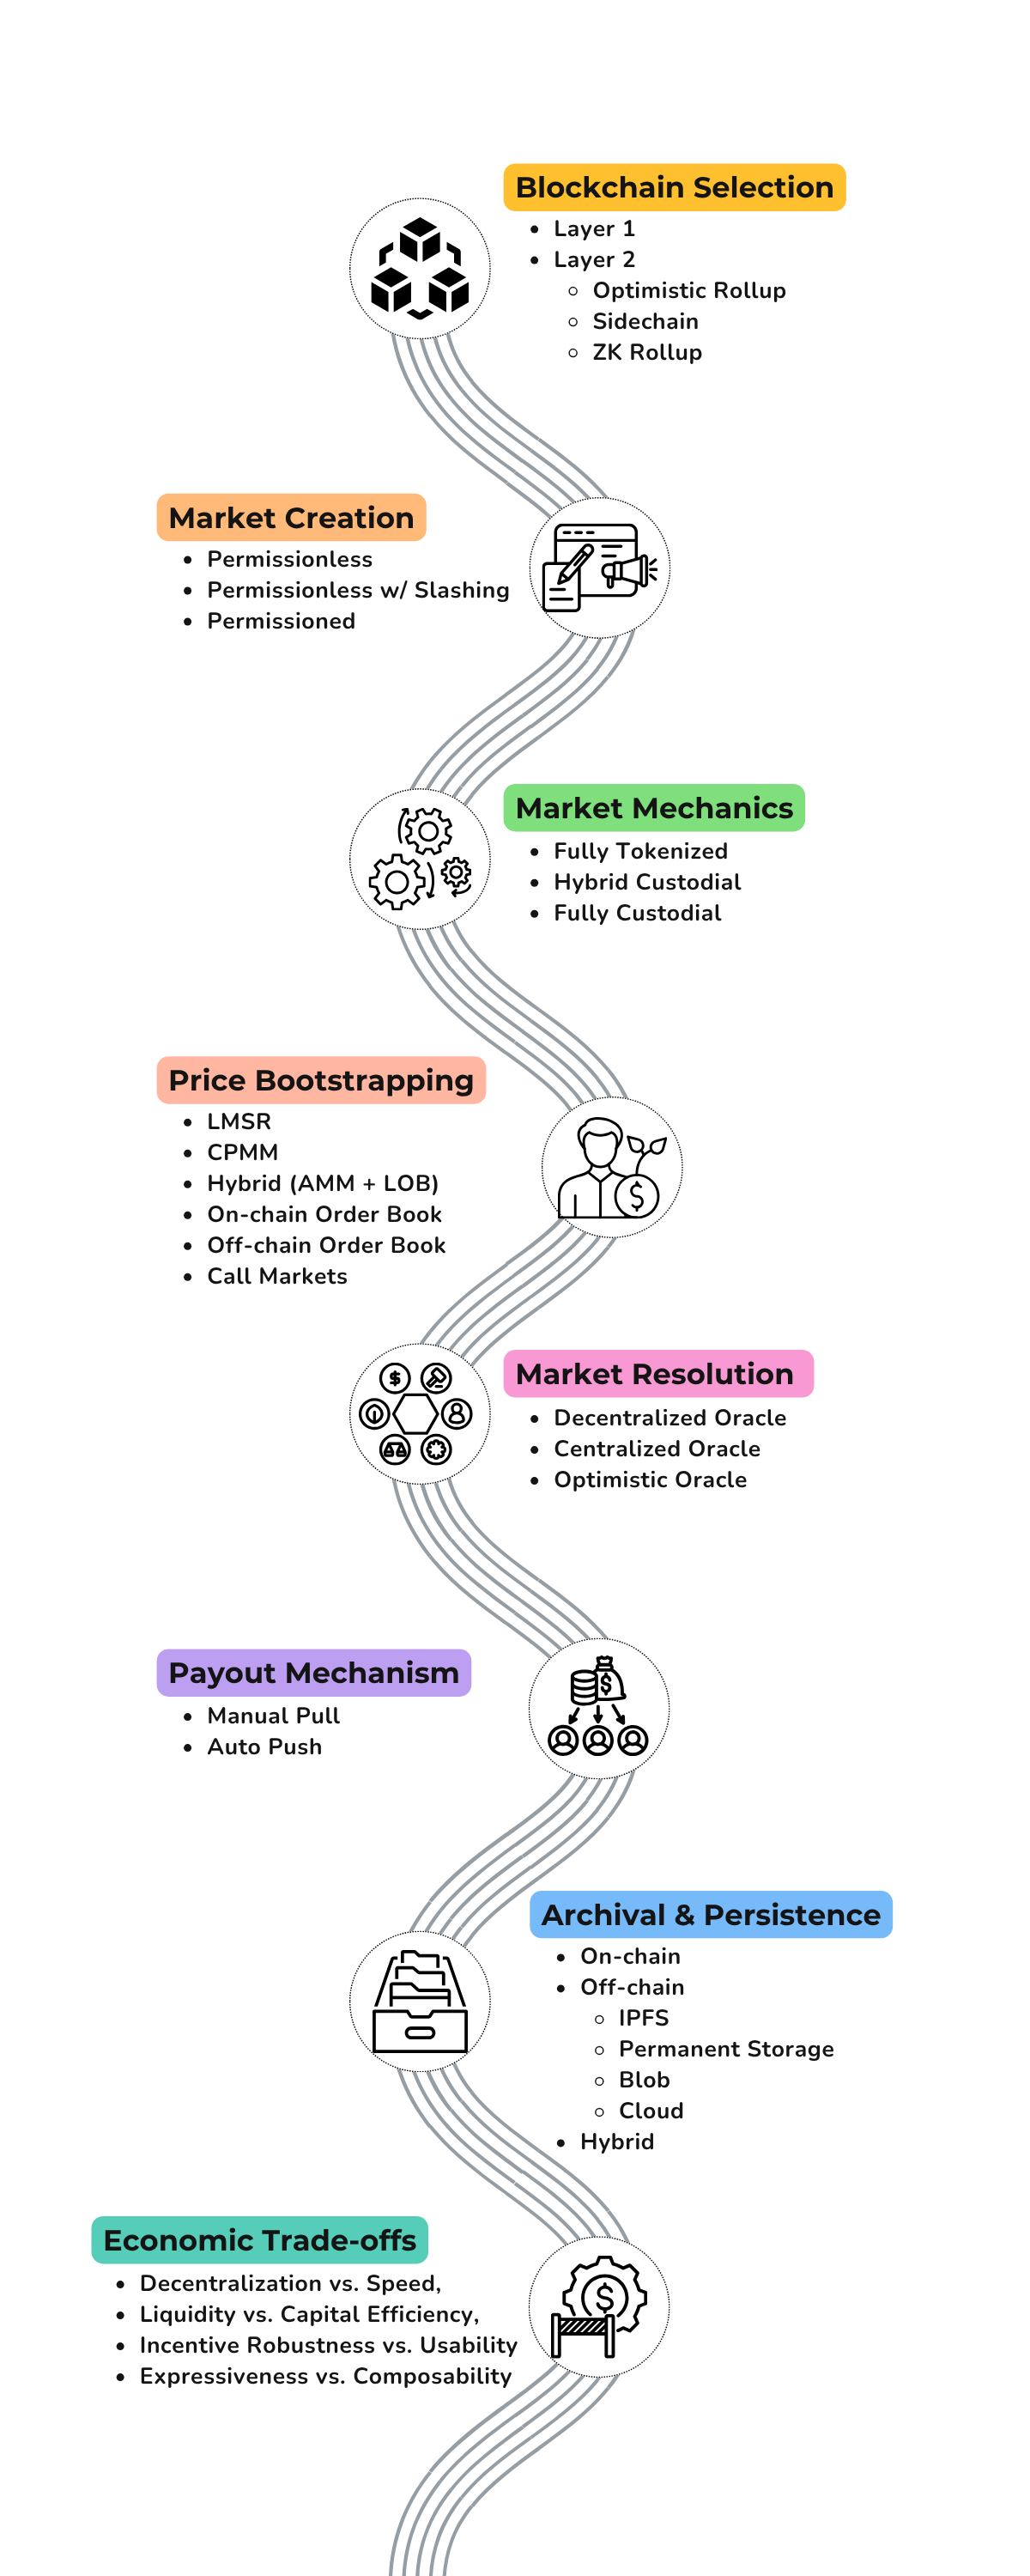
\includegraphics[height=1\textheight]{figures/fig_modular_workflow.png}
%    \caption{Modular Workflow for Decentralized Prediction Market Platforms.}
%    \label{fig:dpm_workflow}
%\end{figure}

\subsection{Underlying Blockchain Infrastructure}\label{subsec:blockchain_infra}
The base blockchain layer (Layer-1 vs. Layer-2) impacts transaction fees, finality guarantees, throughput, and censorship resistance for DPMs, influencing the efficiency and reliability of each stage within the DPM modular workflow. Selecting the underlying blockchain infrastructure constitutes the initial design decision within the modular workflow for DPMs.

Ethereum Layer-1 (L1) mainnet uses proof-of-stake consensus with explicit finality at approximately 13-minute intervals post-Merge, incurring transaction fees typically between \$1 and \$20 and supporting throughput of around 15--30 transactions per second (TPS)~\cite{ClEsGS21}. The relatively higher fees and limited throughput can restrict frequent trading activities and real-time market responsiveness within the DPM modular workflow.

Bitcoin's proof-of-work consensus results in probabilistic finality, generally confirmed after around 60 minutes, with throughput around 7 TPS and fees from \$1 to \$5, impacting the settlement timing and reliability of outcome reporting and payouts in DPMs~\cite{BCFKMN14}. Ethereum's implementation of proposer/builder separation (PBS) and fair-ordering protocols addresses maximal extractable value (MEV) risks, mitigating transaction front-running and block reordering threats that could compromise fairness within market trading and resolution stages~\cite{BBDGJKLZ19}.

Layer-2 (L2) solutions, including optimistic and Zero Knowledge (ZK) rollups, reduce fees to few cents per transaction and improve throughput to thousands of TPS, facilitating high-frequency trading and timely market resolution. Optimistic rollups introduce withdrawal delays of around 7 days due to fraud-proof verification, complicating liquidity management and affecting timely payouts in the market settlement stage. ZK rollups, using validity proofs, offer quicker withdrawal options, beneficial for improving liquidity availability in the workflow~\cite{AKN21}. However, the centralization of sequencers in some L2 platforms like Arbitrum introduces potential censorship issues, partially mitigated by reducing forced-inclusion delays from 24 to 4 hours, thereby influencing market openness and fairness during trading and settlement phases~\cite{BNCD17}.

Bitcoin’s simpler architecture provides resistance to blockchain reorganizations but lacks detailed MEV mitigation, potentially exposing prediction markets to transaction ordering vulnerabilities. Bridging infrastructure connecting L1 and L2 platforms introduces additional latency, complexity, and security risks, potentially disrupting seamless market transitions between layers. Multisig custodians and relay validators involved in bridging have historically been susceptible to financial exploits, highlighting critical risks to asset safety and liquidity flow within the modular workflow of DPMs.

Table \ref{tab:blockchain_infra} below summarizes the performance and decentralization characteristics of blockchain infrastructures relevant to the DPM modular workflow. These infrastructure characteristics shape the feasibility of subsequent market design elements, including market setup and initialization.

\begin{table}[htbp]
    \centering
    \caption{Comparative Attributes of Blockchain Infra for DPM Platforms}
    \begin{tabular}{
        |p{3.2cm}|
        >{\centering\arraybackslash}p{3.2cm}|
        >{\centering\arraybackslash}p{3.2cm}|
        >{\centering\arraybackslash}p{3.2cm}|
     }
         \hline \textbf{Attribute} & \textbf{Ethereum Mainnet} & \textbf{Polygon} & \textbf{Bitcoin} \\
         \hline Transaction Latency & $\sim$12--15 sec/block; \newline $\sim$13 min finality & $\sim$2--5 sec/block & $\sim$10 min/block; \newline $\sim$60 min finality \\
         \hline Bridging Delays & $\sim$7 days \newline (Optimistic Rollups) & $\sim$30 min--3 hrs \newline (Checkpointing) & $\sim$60 min \newline (Sidechains) \\
         \hline Transaction Costs & High \newline (\$1--20+ per tx) & Very low \newline (\$0.01--0.05 per tx) & Moderate-high \newline (\$1--5+ per tx) \\
         \hline Throughput (TPS) & $\sim$15--30 TPS & $\sim$7,000 TPS (peak) & $\sim$7 TPS \\
         \hline Validator Decentralization & High \newline ($\sim$600,000 validators) & Moderate \newline ($\sim$100--150 validators) & High \newline (large miner base) \\
         \hline Censorship Resistance & High \newline (MEV risk present) & Moderate \newline (checkpoint risk) & High \newline (minimal MEV risk) \\
         \hline
    \end{tabular}
    \label{tab:blockchain_infra}
\end{table}

Explicit finality mechanisms, such as Ethereum’s proof-of-stake consensus, provide certainty regarding transaction irreversibility after a specific period, enabling precise timing for market settlements and payouts~\cite{ClEsGS21}. In contrast, probabilistic finality, characteristic of Bitcoin’s proof-of-work, introduces uncertainty, requiring multiple block confirmations, thereby delaying final market outcomes and associated payout distributions~\cite{BCFKMN14}.

\subsection{Market Setup and Initialization}\label{subsec:market_setup_init}
Market setup and initialization choices influence censorship resistance, regulatory compliance, and operational effectiveness of DPMs.

\paragraph{Permissionless Models:} In permissionless setups, such as Augur, any user can initiate markets without centralized oversight, enabling maximum censorship resistance and innovation~\cite{Du19}. This openness creates potential regulatory challenges, illustrated by Augur's "assassination markets" controversy, where third-party moderation efforts (e.g., Predictions.Global) were limited in effectiveness. Economic penalties like validity and no-show reporter bonds address malicious or ambiguous market creation. Permissionless setups typically encourage standardized event templates to minimize ambiguity, though custom markets remain allowed. Collateral selection often involves endogenous (native) tokens (e.g., ETH for Augur), introducing volatility risk and regulatory complexity, balanced by potential hedging benefits when outcomes correlate with token value~\cite{AKPWZ19}~\cite{Sz15}.

\paragraph{Hybrid Governance Models (Permissionless with Centralized Slashing):} Hybrid models allow permissionless market creation combined with centralized oversight mechanisms. Platforms like Polymarket use entities such as a Market Integrity Committee to enforce compliance and penalize markets violating rules~\cite{ClEsGS21} ~\cite{Du19}. This partially decentralizes market listing but maintains centralized control, creating regulatory accountability and single points of control. Hybrid platforms also leverage standardized event templates to maintain clarity and reduce dispute risk, supplemented by custom market oversight. Collateral choices generally include stablecoins, reducing volatility exposure and regulatory uncertainty compared to endogenous tokens.

\paragraph{Permissioned Models:} Fully permissioned setups, including Kalshi and PredictIt, require internal or regulatory reviews before listing markets, significantly reducing regulatory and operational risks by limiting ambiguous or unlawful markets ~\cite{BCFKMN14}. Market proposals typically use standardized event templates to ensure unambiguous resolution, supported by rigorous internal review. Collateral is generally stablecoins or fiat currency, minimizing volatility and simplifying regulatory compliance. Strict implementation of KYC/AML protocols further reduces regulatory exposure, though it introduces operational overhead and restricts market diversity~\cite{Du19}.

Table \ref{tab:market_setup_init} summarizes operational implications for each market setup, guiding stakeholders in selecting appropriate governance models based on desired censorship resistance, compliance requirements, and collateral management.

\begin{table}[htbp]
     \centering
     \caption{Comparative Evaluation of Market Creation and Permission Models}
     \begin{tabular}{
         |p{2.6cm}|
         >{\centering\arraybackslash}p{4.3cm}|
         >{\centering\arraybackslash}p{3.4cm}|
         >{\centering\arraybackslash}p{2.5cm}|
     }
         \hline \textbf{Market Setup} & \textbf{Benefits} & \textbf{Drawbacks} & \textbf{Platforms} \\
         \hline Permissionless & Open participation, censorship resistance, flexible collateral (endogenous tokens) & Regulatory risks, potential misuse, collateral volatility exposure & Augur, PlotX, Gnosis \\
         \hline Permissionless with Slashing & Openness balanced by centralized enforcement, stable collateral (stablecoins) & Centralized oversight, regulatory accountability & Polymarket, UMA\textsuperscript{*} \\
         \hline Permissioned & Compliance, controlled market environment, stable collateral (stablecoins, fiat) & Limited diversity, lower censorship resistance, operational overhead & Kalshi, PredictIt, Stox \\
         \hline
    \end{tabular}
    \label{tab:market_setup_init}
    \vspace{0.5em}
    {\footnotesize\textsuperscript{*}UMA is not a DPM in the traditional sense; it is mentioned here due to its Permissionless with Slashing model usage.}
\end{table}

\subsection{Market Mechanics and Share Custodianship}\label{subsec:market_mechcanics}
Market mechanics and share custodianship directly influence the operational efficiency, liquidity, and decentralization of DPMs.

Binary markets offer intuitive simplicity and consolidated liquidity, facilitating hedging via straightforward YES/NO token pairs, as exemplified by Polymarket’s ERC-1155 tokens redeemable for \$1 upon outcome resolution~\cite{AKPWZ19} ~\cite{IOSG20} This binary structure enables users to hedge risks akin to insurance instruments, although extensive hedging activities by risk-averse participants can temporarily distort prices, potentially diverging from true event probabilities until arbitraged by informed traders~\cite{Ha03}.

In contrast, combinatorial markets, which enable complex bets on interdependent outcomes, significantly enhance theoretical information aggregation by capturing correlations and conditional probabilities but impose exponential computational complexity (\#P-hard for LMSR market makers) and cognitive burdens on users~\cite{CFLPW08}~\cite{CP10}. Thus, combinatorial markets have remained largely experimental, given the difficulty in matching trades efficiently without algorithmic support and substantial fragmentation of liquidity (Pennock \& Sami, 2007).

Markets inherently start with zero traders, necessitating careful liquidity bootstrapping to avoid under-collateralization and price manipulation. Safe market initialization requires at least two traders with opposing views (or one trader matched by an automated market maker) to create balanced, fully collateralized initial positions. This balanced issuance is critical to avoid under-collateralization and ensure meaningful initial price discovery; for instance, Polymarket only mints YES and NO shares simultaneously upon matched buyer-seller orders that sum exactly to \$1 collateral ~\cite{BCFKMN14}. Similarly, Augur mandates traders to initially collateralize all outcomes fully, thus guaranteeing solvent market conditions from inception~\cite{AKPWZ19}.

Custodianship models significantly affect decentralization, regulatory visibility, and systemic trust. Fully tokenized on-chain shares (ERC-20/ERC-1155) maximize decentralization and composability within broader DeFi ecosystems. Conversely, centralized custodial models, though enabling simpler KYC/AML integration, inherently risk censorship and unilateral asset control, undermining core decentralized principles~\cite{Du19}. Polymarket notably adopted more centralized custodianship following regulatory enforcement by the CFTC, underscoring the practical impacts of regulatory pressures on market design~\cite{Ma24}.
Table \ref{tab:market_mechcanics} below summarizes custodianship models, highlighting their implications for composability, decentralization, and systemic trust.

\begin{table}[htbp]
    \centering
     \caption{Comparative Analysis of Custody Models for Outcome Tokenization}
     \begin{tabular}{
         |p{2.7cm}|
         >{\centering\arraybackslash}p{2.5cm}|
         >{\centering\arraybackslash}p{2.8cm}|
         >{\centering\arraybackslash}p{3cm}|
         >{\centering\arraybackslash}p{2cm}|
         >{\centering\arraybackslash}p{2.5cm}|
     }
          \hline \textbf{Custody Model} & \textbf{Composability} & \textbf{Regulatory Visibility} & \textbf{Systemic Trust \& Risk} & \textbf{Decentralization} & \textbf{Examples} \\
          \hline Fully Tokenized (ERC-20 / ERC-1155) & High (DeFi interoperability) & High (public) & Smart-contract reliant & High & Augur, Gnosis \\
          \hline Hybrid Custodial & Moderate & Moderate-high (KYC/AML) & Partial central reliance & Moderate & Polymarket, UMA \\
          \hline Fully Centralized & Low (none) & Low visibility, high control & Centralized, censorship risk & Low & Kalshi, PredictIt \\
          \hline
     \end{tabular}
     \label{tab:market_mechcanics}
\end{table}

\subsection{Price Bootstrapping and Liquidity Mechanisms}\label{subsec:price_bootstrapping}
Price bootstrapping and liquidity provision enable initial price formation and continuous trading in DPMs. Automated Market Makers (AMMs) address the bootstrapping challenge by providing immediate liquidity and initial price setting without requiring initial trading counterparties.
The Logarithmic Market Scoring Rule (LMSR), introduced by~\cite{Ha03}, utilizes a convex cost function:
FORMULA REMOVED
	where b>0 defines liquidity depth~\cite{OPRS13}.
LMSR adjusts instantaneous outcome prices using a softmax function to maintain valid probability distributions. LMSR limits liquidity provider losses to a maximum of \( b \ln{N} \) for a market with N outcomes, providing a known loss boundary~\cite{CP10}.
Selecting the liquidity parameter b presents practical challenges; inappropriate values can result in either excessive price sensitivity or limited market responsiveness~\cite{Ha03}.
Constant Product Market Makers (CPMM), such as those based on the invariant:
\[x \cdot y = k\]

manage liquidity by holding two token reserves, with outcome prices determined by the ratio of these reserves~\cite{AC20}. Arbitrage ensures prices generally sum to a valid probability distribution. However, CPMMs expose liquidity providers to divergence loss (impermanent loss), where large shifts in outcome probabilities leave providers holding primarily the less valuable tokens at resolution~\cite{CDM23}. Unlike LMSR, CPMM does not limit potential losses, thus introducing additional financial risk despite operational simplicity and compatibility with decentralized finance (DeFi) protocols.
Hybrid models integrating AMMs with limit order books (LOBs), as implemented by platforms like Polymarket, combine continuous liquidity provided by AMMs with liquidity precision offered by order books~\cite{ClEsGS21}. These hybrid systems facilitate arbitrage-driven adjustments that stabilize market prices and maintain accurate probability reflections, balancing AMM simplicity with order book responsiveness.

Alternative liquidity mechanisms, including pure on-chain order books and periodic call markets, introduce distinct trade-offs, which are detailed in Table 1. Pure on-chain order books offer precise pricing but encounter issues related to transaction latency and high gas fees, whereas off-chain order books mitigate these problems at the expense of decentralization ~\cite{BCFKMN14}. Call markets aggregate trades at regular intervals to improve liquidity but face latency issues and potential arbitrage vulnerabilities due to delayed execution~\cite{ACES17}.

Table \ref{tab:price_bootstrapping} contrasts liquidity mechanisms used in decentralized prediction markets by evaluating their risk characteristics, price formation methods, and operational attributes. Each mechanism presents unique trade-offs, balancing liquidity provider risks, system complexity, arbitrage vulnerabilities, and operational efficiency.

\begin{table}[htbp]
    \centering
    \caption{Comparative Analysis of Liquidity Mechanisms}
    \begin{tabular}{
        |p{3cm}|
        >{\centering\arraybackslash}p{1.6cm}|
        >{\centering\arraybackslash}p{2.5cm}|
        >{\centering\arraybackslash}p{2cm}|
        >{\centering\arraybackslash}p{2.3cm}|
        >{\centering\arraybackslash}p{2.7cm}|
    }
        \hline \textbf{Liquidity Mechanism} & \textbf{Loss Limitation} & \textbf{Price Formation} & \textbf{Complexity} & \textbf{Arbitrage Exposure} & \textbf{Operational Latency} \\
        \hline LMSR & Yes & Softmax pricing & Moderate & Moderate & Low \\
        \hline CPMM & No & Reserve ratios & Low & High & Low \\
        \hline Hybrid (AMM + LOB) & Partial & Mixed & High & Moderate & Low to Moderate \\
        \hline On-chain Order Book & No & Order matching & High & Moderate & High \\
        \hline Off-chain Order Book & No & Order matching & Moderate & Moderate & Low \\
        \hline Call Markets & No & Batch matching & Moderate & High & Moderate to High \\
        \hline
   \end{tabular}
   \label{tab:price_bootstrapping}
\end{table}

\subsection{Market Resolution and Dispute Models}\label{subsec:market_resolution}
Market resolution and dispute models are essential for accurate and fair settlement in DPMs, directly affecting market credibility and operational continuity.
Single-trusted entity models utilize a single oracle, such as the Associated Press, enabling efficient and rapid finalization. However, reliance on a single entity introduces centralization risks, including vulnerability to bribery and biased reporting~\cite{ClEsGS21}. Economic deterrents like escrow bonds may not prevent manipulation if potential gains surpass the penalties.

Decentralized oracle collectives distribute decision-making across multiple oracles. Chainlink aggregates data from independent nodes using median or majority votes, with nodes required to stake tokens, incentivizing accuracy and penalizing errors. MakerDAO uses governance-based collectives, electing trusted data feeders through community governance to enhance transparency and reduce individual collusion risks~\cite{ClEsGS21}. These collectives, however, experience higher latency and complexity and remain susceptible to coordinated manipulation and governance capture. UMA’s Data Verification Mechanism (DVM) dynamically calculates stakes based on the Cost of Corruption versus Profit from Corruption, aiming to ensure corruption costs always exceed potential profits~\cite{CLL19}. Realitio employs a tiered dispute escalation process, resolving uncontested outcomes swiftly while disputed cases escalate to external arbitrators like Kleros, balancing speed and decentralization.

Self-settling models depend entirely on internal incentives to align reporter behaviour around Schelling points. Augur exemplifies this, with REP tokens staked to encourage reporting consistent with the majority's expectations. Disputes trigger increased staking requirements and potentially protocol forks, reinforcing truthful reporting through economic incentives~\cite{AKPWZ19}. Yet, these mechanisms are vulnerable to coordinated bribery and external manipulation, especially when attackers exploit side-bet strategies~\cite{BF19}. An attacker-defender payoff matrix clearly illustrates these economic vulnerabilities, highlighting equilibrium conditions shaped by manipulation costs and incentives.

Table \ref{tab:market-resolution-types} provides a comparative evaluation of oracle types, outlining operational characteristics, specific risks, and representative examples. It succinctly differentiates between single trusted entities, decentralized oracle collectives, and self-settling oracles by highlighting advantages such as decentralization levels and inherent vulnerabilities like susceptibility to bribery.

\begin{table}[htbp]
    \centering
    \caption{Comparative Evaluation of Market Resolution Types}
    \begin{tabular}{
        |p{3.5cm}|
        >{\centering\arraybackslash}p{3.5cm}|
        >{\centering\arraybackslash}p{3.8cm}|
        >{\centering\arraybackslash}p{3.5cm}|
    }
       \hline \textbf{Oracle Type} & \textbf{Pros} & \textbf{Cons} & \textbf{Examples} \\
       \hline Single Trusted Entity & Fast resolution; clear accountability & Single failure point; high censorship risk & Associated Press, Chainlink \\
       \hline Decentralized Oracle Collective & Distributed trust; censorship resistance & Higher complexity; risk of collusion & UMA, Realitio, MakerDAO \\
       \hline Self-Settling (Schelling-Point) & No external trust; economic incentives & Vulnerable to bribery; fork complexity & Augur, Truthcoin, Kleros \\
       \hline
     \end{tabular}
     \label{tab:market-resolution-types}
\end{table}

Table \ref{tab:oracle-payoff-matrix} presents a detailed incentive compatibility payoff matrix for Augur’s REP staking mechanism. It describes four distinct situations with different combinations of attacker and honest stakes, and potential rewards if an attacker succeeds versus consequences if defenders successfully prevent the attack. The first scenario shows stability when no attack occurs and reporting remains honest, generating standard rewards. In the second scenario, a small attacker stake versus a larger honest stake renders attacks unlikely due to limited attacker profitability. However, in scenarios with higher attacker stakes or significant external bets, the table demonstrates potential attacker profitability, making bribery economically viable and possibly leading to the breakdown of the Schelling point equilibrium.

\begin{table}[htbp]
    \centering
    \caption{Oracle Incentive Compatibility Payoff Matrix (Example: Augur REP Game)}
    \begin{tabular}{
        |p{3.2cm}|
        >{\centering\arraybackslash}p{2cm}|
        >{\centering\arraybackslash}p{1.6cm}|
        >{\centering\arraybackslash}p{2.2cm}|
        >{\centering\arraybackslash}p{2.6cm}|
        >{\centering\arraybackslash}p{3cm}|
    }
        \hline \textbf{Scenario} & \textbf{Attacker Stake (A)} & \textbf{Honest Stake (H)} & \textbf{Attacker Reward if Successful} & \textbf{Defender Reward if Successful} & \textbf{Equilibrium Result} \\
        \hline No Attack, Honest Majority & \$0 & \$1,000,000 & \$0 & \$0 \newline (normal fees) & Honest Reporting Stable \\
        \hline Attack, Low Attacker Stake & \$500,000 & \$1,000,000 & \$10,000,000 & Attacker's stake \newline (slashed) & Honest Reporting Stable \newline (Attack Unlikely) \\
        \hline Attack, High Attacker Stake & \$1,500,000 & \$1,000,000 & \$10,000,000 & Attacker's stake \newline (slashed) & Attacker Profitable \newline (Bribe Possible) \\
        \hline Coordinated Side-Bet Bribery & \$2,000,000 & \$1,000,000 & \$20,000,000 \newline (external bets) & Attacker's stake \newline (slashed) & Attack Profitable \newline (Schelling Point Fails) \\
        \hline 
    \end{tabular}
    \label{tab:oracle-payoff-matrix}
\end{table}



To mitigate vulnerabilities identified in Table 6, designers can implement thresholds for stake escalation and require proportionally larger attacker stakes relative to honest stakes to disrupt equilibrium~\cite{AKPWZ19}. Additionally, periodic audits or community-based moderation processes may deter coordinated attacks, reinforcing equilibrium stability~\cite{ClEsGS21}.

\subsection{Payout and Redemption Mechanisms}\label{subsec:payout_redemption}
DPMs commonly implement push or pull payout mechanisms, each presenting distinct trade-offs. Push payout models automatically distribute winnings once market outcomes are resolved, reducing user interaction requirements. However, they face scalability and cost constraints due to increased gas usage, especially in scenarios involving numerous recipients~\cite{ClEsGS21}. Polymarket uses a hybrid model on the Polygon network with USDC that mimics push mechanisms via meta-transactions, effectively removing direct user gas fee payments~\cite{Ma24} Castle Capital, 2024). Conversely, Augur utilizes a pull mechanism, requiring users to manually redeem tokens to collect payouts. This approach prioritizes decentralization but increases the complexity and cost associated with claiming rewards~\cite{AKPWZ15}.

Gasless redemption mechanisms aim to improve usability by eliminating user gas fees, typically relying on third-party relayers to cover transaction costs. Such mechanisms enhance accessibility but introduce dependencies on centralized components, creating potential points of failure or censorship (Castle Capital, 2024).

Time-bounded redemption windows set deadlines for payout claims, aiming to reduce inefficiencies caused by permanently locked collateral. These mechanisms can enhance capital utilization but raise ethical and regulatory concerns, including issues related to unclaimed property regulations and user fairness~\cite{ClEsGS21}. Major platforms like Augur and Polymarket generally favor open-ended claims to uphold continuous user rights.

Surplus management deals with residual funds from unclaimed or locked winnings. Permanent locking maintains explicit user ownership at the expense of economic efficiency over time, exemplified by Augur’s approach~\cite{ClEsGS21}. Redistribution methods periodically allocate surplus to liquidity providers or active users, increasing capital efficiency but potentially creating incentives to abandon minor balances intentionally. Governance-controlled treasuries allow directed surplus management, balancing efficiency against the risk of centralized governance influence and regulatory attention~\cite{BMR17}.

Table \ref{tab:surplus-management} compares surplus management methods in decentralized prediction markets, evaluating their economic efficiency, ethical considerations, and regulatory implications. It identifies trade-offs between preserving explicit user ownership and maximizing capital efficiency, highlighting potential governance risks and compliance requirements for different mechanisms.

\begin{table}[htbp]
    \centering
    \caption{Comparative Evaluation of Surplus Management Mechanisms}
    \begin{tabular}{
        |p{2.5cm}|p{3.8cm}|
        >{\centering\arraybackslash}p{2cm}|
        >{\centering\arraybackslash}p{2.5cm}|
        >{\centering\arraybackslash}p{2.5cm}|
        >{\centering\arraybackslash}p{2.5cm}|
    }
        \hline \textbf{Mechanism} & \textbf{Description} & \textbf{Economic Efficiency} & \textbf{Ethical Considerations} & \textbf{Regulatory Implications} & \textbf{Example Platforms} \\
        \hline Permanent Locking & Surplus funds locked indefinitely post-resolution & Low & Maintains explicit user ownership & Low regulatory risk & Augur, Gnosis \\
        \hline Redistribution to LPs/Stakers & Surplus periodically redistributed to liquidity providers & High & May incentivize intentional abandonment & Moderate, potential property concerns & UMA, Realitio \\
        \hline Governance-controlled Treasury & Surplus directed by governance structures & Moderate–High & Potential governance influence risk & Moderate–High, regulatory attention & Polymarket, SX Network \\
        \hline Burning Tokens & Surplus tokens destroyed to reduce supply & Moderate–High & Minimal ethical concerns & Moderate, regulatory stance uncertain & Truthcoin (theoretical) \\
        \hline Returning to Original Funders & Surplus returned to initial market creators & Moderate & Risks manipulation incentives & High, KYC and AML compliance concerns & Kalshi \\
        \hline
    \end{tabular}
    \label{tab:surplus-management}
\end{table}

\subsection{Archival, Transparency, and Meta-Data Persistence}\label{subsec:archival}
Archival, transparency, and metadata persistence within DPMs ensure verifiable and accessible records, directly impacting market integrity and governance processes.

Critical metadata, such as market states, transaction histories, and resolution outcomes, inherently benefit from blockchain immutability and cryptographic verification~\cite{Du19},~\cite{ClEsGS21}. Augur v2 stores metadata, including user profit/loss computations, directly on-chain, providing immediate access without external archives. This design increases transparency but also results in higher transaction costs and larger blockchain state size~\cite{Fo20}.

Off-chain metadata - including market descriptions, resolution criteria, and user-generated content - are typically stored in decentralized storage solutions due to blockchain capacity constraints~\cite{BCCJM21}. IPFS (InterPlanetary File System) employs peer-to-peer, content-addressable storage using cryptographic hashes, verifying content authenticity through immutable identifiers. IPFS’s availability depends on node operators maintaining persistent storage through pinning, without central points of failure~\cite{IM24}. Arweave offers an economic incentive structure combined with a "blockweave" architecture for permanent data storage, providing perpetual availability and resistance to censorship~\cite{BCKW23}.

Recent updates to Ethereum, such as proto-danksharding, provide ephemeral "blob" storage. These storage blobs temporarily allow for large metadata availability and cryptographic verification. However, their short-term nature necessitates subsequent migration to persistent storage solutions~\cite{Fo20}.

The archival model chosen by a DPM influences governance outcomes and resilience against manipulation. Persistent archival supports retrospective audits critical for resolving disputes and maintaining accountability of oracle activities~\cite{ClEsGS21}. Decentralized archival mechanisms prevent centralized control from suppressing or altering market data, enabling community-driven governance or protocol forks when required~\cite{BCKW23}.

Table \ref{tab:archival-methods} compares archival methods such as blockchain storage, IPFS, Arweave, Ethereum blob storage, and hybrid models. It details each method's durability, authenticity, and accessibility, highlighting their distinct operational trade-offs and cost implications for decentralized prediction markets.

\begin{table}[htbp]
    \centering
    \caption{Comparative Evaluation of Archival Methods for Decentralized Prediction Markets}
    \renewcommand{\arraystretch}{1.3}
    \begin{tabular}{
        |p{2.3cm}|
        p{3cm}|
        >{\centering\arraybackslash}p{2.0cm}|
        >{\centering\arraybackslash}p{2.5cm}|
        >{\centering\arraybackslash}p{2.8cm}|
        >{\centering\arraybackslash}p{2.6cm}|
    }
        \hline \textbf{Archival Method} & \textbf{Description} & \textbf{Durability \& Persistence} & \textbf{Authenticity \& Integrity} & \textbf{Accessibility \& Discovery} & \textbf{Example Platforms} \\
        \hline Blockchain On-chain Storage & Directly store metadata and outcomes on-chain (e.g., Ethereum). & Extremely high (immutable, perpetual) & High authenticity (cryptographic guarantees) & Excellent (immediate, global nodes) & Augur (partial), Gnosis \\
        \hline IPFS (InterPlanetary File System) & Decentralized, peer-to-peer, content-addressable storage. & Medium (requires community pinning) & High (content hashes provide tamper-evidence) & Good (distributed nodes, variable retrieval speeds) & Augur, Polymarket \\
        \hline Arweave Permanent Storage & Blockchain-based storage with economic incentives for permanent retention. & Very high (economically incentivized permanence) & Very high (blockchain-backed immutability) & High (permanent, redundant node distribution) & Mirror.xyz, RedStone Oracles (experimental) \\
        \hline Ethereum Blob Storage & Temporary large-data storage via Ethereum blobs (proto-danksharding). & Low (temporary, ephemeral data availability) & High (cryptographic authenticity guaranteed short-term) & Moderate (short-term retrieval from Ethereum nodes) & Ethereum L2s (Optimism, Arbitrum) \\
        \hline Centralized Cloud Storage & Traditional cloud services (AWS, Google Cloud). & Variable (single point of failure risk) & Low–moderate (trust reliant on centralized operator) & High (fast retrieval, easy indexing) & Early centralized prediction platforms \\
        \hline Hybrid Storage Model & Combination: blockchain on-chain pointers plus decentralized or permanent storage. & High (leverages strengths of multiple methods) & High (on-chain hashes guarantee authenticity) & Very high (multiple redundancy points, robust discovery) & Polymarket, UMA \\
        \hline
    \end{tabular}
    \label{tab:archival-methods}
\end{table}

\subsection{Economic Trade-Offs in DPM Design}\label{subsec:economic_tradeoff}
The design of DPMs involves inherent economic trade-offs affecting platform adoption, integrity, and resilience. This analysis examines these trade-offs across four dimensions: decentralization versus speed, liquidity versus capital efficiency, incentive robustness versus usability, and expressiveness versus composability, with agility noted as an additional consideration.

A fundamental trade-off occurs between decentralization and execution speed. Fully decentralized DPMs, such as early Augur versions, achieve censorship resistance but experience latency and high transaction costs due to reliance on Ethereum’s mainnet~\cite{BCFKMN14}~\cite{AKPWZ15}. Hybrid models, including Polymarket, employ off-chain order matching and on-chain settlements or dedicated sidechains to increase throughput and improve usability, albeit with the addition of trust assumptions and centralization risks~\cite{ClEsGS21}. Layer-2 technologies like state channels and rollups offer alternative methods to balance decentralization and performance~\cite{BBMMM19}.

Liquidity provision versus capital efficiency presents another critical trade-off. Automated market makers (AMMs), such as Hansonian market scoring rules or constant product market makers (CPMM), deliver continuous liquidity by committing substantial collateral, reducing capital efficiency~\cite{Ha03}~\cite{AC20}. Conversely, order-book-based models maximize capital efficiency by avoiding idle capital but can encounter liquidity issues and impaired price discovery, as noted in Augur v1 markets~\cite{AA20}. Platforms like Gnosis address some of these challenges through conditional markets that dynamically allocate capital among outcomes~\cite{Gn17}.

Incentive robustness and usability reflect another key trade-off. Augur’s multi-stage dispute mechanisms and token staking enhance manipulation resistance but complicate user experience and slow resolution processes~\cite{AKPWZ15}~\cite{ClEsGS21}. In contrast, simplified oracle solutions, such as UMA's optimistic oracle, offer streamlined resolution processes but carry greater risks of manipulation. Hierarchical or two-tiered dispute frameworks (e.g., Pisa watchtowers) seek to address these issues by maintaining manipulation resistance while minimizing complexity~\cite{BBMMM19}.

Expressiveness versus composability represents an additional design dimension. Highly expressive combinatorial market structures, such as those enabled by Gnosis’s Conditional Tokens, allow detailed market configurations but reduce interoperability and composability with other decentralized finance (DeFi) systems due to technical complexity~\cite{Gn17}. Simpler binary or categorical markets increase interoperability and composability but sacrifice detailed market structuring capabilities.





% !TEX root = ../main.tex

\section{List of \depms}
\label{app:list}

 %Terminology used includes a central limit order book (CLOB) in which `central' refers to a single orderbook rather than one that is centralized from an operational standpoint. In other words, a decentralized on-chain orderbook can still be called a CLOB. Blockchains are sometimes called layer 1 (L1) chains. An L2 is a faster execution (and generally lower fee) layer that might operate as an optimistic rollup or zk-rollup. An L3... 

\begin{enumerate}

\item \textbf{Bets of Bitcoin} (2011--2014): Centralized event wagering system with BTC as numeraire. Promoted as a prediction market but mechanically it used parimutuel betting. Went offline unannounced with some user funds stuck.

\item \textbf{BitBet} (2012--2020): Centralized event wagering system with BTC as numeraire. Promoted as a prediction market but mechanically it used parimutuel betting. Disruption in 2016 and winddown in 2020. 

\item \textbf{Predictious} (2013--?): Centralized prediction market and CLOB with BTC as numeraire. Promoted as InTrade successor. Appears abandoned in late 2010s.

\item \textbf{Fairlay} (2014--present): Centralized prediction market with BTC as numeraire. Traders were matched on a CLOB (back/lay mechanism). After ownership changes, still operating as Bitcoin Betting. 

\item \textbf{BetMoose} (2014--present) Centralized event wagering system with BTC as numeraire. Promoted as a prediction market but mechanically it used parimutuel betting or back/lay. Still active. 

\item \textbf{Truthcoin / Bitcoin Hivemind} (2014): Decentralized prediction market (\depm) design with follow-up refinements with some code artifacts. Inspired other \depms (particularly around automated book making and token vote market resolution) and sidechain technologies.

\item \textbf{`Princeton' \depm} (2014): Decentralized prediction market (\depm) design as an academic paper only. Inspired other \depms (particularly around share splitting/merging), on-chain CLOBs (frequent batch auctions) and the concept of MEV.  

\item \textbf{Augur} (2015--present): \depm whitepaper design, later deployed on Ethereum (live in 2018) and Polygon (2021). Numeraire is DAI and later USDC. Native token (REP) used in market resolution was one of Ethereum's first ICOs (2015). Still active. Alternative front-ends for Augur include \textbf{Veil}, \textbf{Gueser}, \textbf{Helena Network}, and \textbf{Predictions.Global}.

\item \textbf{BitShares Prediction Markets} (2015--present): \depm functionality was added to the BitShares 2.0 blockchain to support WTA markets and hybrid on/off-chain CLOBs. \depm functionality dormant. BitShares itself is still active but usage has heavily declined.
 
\item \textbf{Gnosis} (2015--present): \depm whitepaper design for Ethereum. Pivoted to developing underlying infrastructure for \depms, including the widely used Conditional Tokens Framework (CTF). Also known for self-custody wallets (Gnosis Safe) and AMM-relevant research (proposing the constant product market maker). Still active. 

\item \textbf{Stox} (2017--2018): Centralized prediction market and CLOB with custom ERC20 token STX as numeraire. Known for celebrity promotions. Abandoned around 2018 after legal issues. 

\item \textbf{Delphy} (2017--?): Prediction aggregator deployed on Ethereum for mobile devices based on points/leaderboard (`play money') rather than money. Appears to have been abandoned within 2-3 years.

\item \textbf{Bodhi} (2017--?): \depm deployed on Qtum blockchain and later Ethereum. Appears to have been abandoned within 2-3 years. 

\item \textbf{BlitzPredict} (2018--2019): Prediction aggregator on Ethereum that appears to have been abandoned before being developed into a full \depm.

\item \textbf{SportX} (2018--): Sports-centric \depm deployed on Ethereum, Polygon, and later its own EVM chain (SX Network). Still active.

\item \textbf{BetProtocol} (2018): Toolkit for \depm infrastructure using custom ERC20 token BEPRO. Bepro Network pivoted in 2021 and no active development on toolkit since.

\item \textbf{Sharpe Capital} (2017--2019): Prediction aggregator on Ethereum that appears to have been abandoned before being developed into a full \depm.

\item \textbf{Amoveo} (\circa 2018--?): \depm functionality into state-channels on a custom PoW L1 chain. Sporadic ongoing development.

\item \textbf{SEER} (2018--?): \depm deployed on custom Graphene-based DPoS L1 chain with custom SEER token as numeraire. Appear abandoned as of 2020.

\item \textbf{Veil} (2019): \depm front-end built on Augur and 0x. Launched and shut down within 2019.

\item \textbf{PredIQt} (2019--?): \depm deployed on EOSIO with IQ/EOS as numeraire. Project pivoted to encyclopedia IQ.wiki and PredIQt appears inactive.

\item \textbf{Catnip.exchange} (2019): \depm front-end for Augur v1 that composed with Balancer AMMs for trading outcome shares. Discontinued after 2020 US presidential election.

\item \textbf{Flux Protocol} (2019--2022): \depm deployed on Ethereum and later NEAR. Appears dormant after 2022. 

\item \textbf{Thales} (2019--2022): Event wagering system deployed on Ethereum and later NEAR. Market resolution with Chainlink. Largely dormant after 2022.

\item \textbf{Omen} (2020--present): \depm built with Gnosis CTF, deployed on Ethereum and later Gnosis Chain (xDai) and Polygon with any ERC20 as numeraire. Market resolution with Reality.eth and Kleros. Still active.

\item \textbf{Polymarket} (2020--present): \depm built with Gnosis CTF, deployed on Polygon with USDC as numeraire. First \depm to receive wide mainstream coverage in the media. Market resolution with UMA. Still active but restricted in some jurisdictions (including the US). 

\item \textbf{PlotX v1} (2020--2022): \depm deployed on Ethereum and later Polygon. Specialized for crypto price predictions. PlotX still active but 2022 pivot left \depm functionality dormant. 

\item \textbf{Reality Cards} (2020--2022): \depm deployed on Ethereum and later Gnosis and Polygon. Outcomes shares are NFTs that can be rented with payouts based on how long a user held the winning NFT (time-weighted to compensate early traders more). Appears abandoned in 2022.

\item \textbf{Prosper} (2021--present): \depm deployed on Avalanche and BSC. Still active.

\item \textbf{Zeitgeist} (2021--present): \depm deployed into the logic of a parachain (custom L1) in the Polkadot/Kusama ecosystem (L0). Still active.

\item \textbf{Polkamarkets} (2021--present): \depm toolkit for EVM chains like Polygon and Moonriver with any ERC-20 as numeraire (and custom ERC20 POLK for governance). Still maintained.

\item \textbf{Hedgehog Markets} (2021--?): Event wagering platform deployed on Solana with USDC as numeraire. Supports both no-loss contests and prediction markets. Appears dormant after 2022.

\item \textbf{Unihedge} (2021): \depm design for EVM with an experimental prototype. Outcomes shares are structured different than a typical prediction market (lots implementing what is known as a Harberger-tax).

\item \textbf{Mojito Markets} (2022--present): \depm designed for Aptos but not yet deployed.

\item \textbf{Insight Prediction} (2024--present): \cepm with blockchain-based payments in various stablecoins, including USDC. Still active.

\item \textbf{Moonopol} (2024--present): \depm deployed on Solana with USDC as numeraire. Still active.

\item \textbf{Miscellaneous}: There are decentralized event wagering systems (or toolkits) that deploy betting structures different from prediction markets. For the earliest systems using such an adjacent approach, we have included them above. However we do not expand on every follow-up project. These include: \textbf{Wagerr}, \textbf{BetDEX}, \textbf{Monaco Protocol}, \textbf{Peerplays}, \textbf{DexWin}, \textbf{DuelDuck}, \textbf{BetterFan}, \textbf{Oriole Insights}, \textbf{BetSwag.gg} and \textbf{Azuro}. We also note here the most prominent \cepms: \textbf{Kalshi}, \textbf{PredictIt}, \textbf{Futuur}, and \textbf{Manifold}. 

\end{enumerate}














\section{Satoshi HBO Market}
\label{app:hbo}

\begin{figure}
  \centering
  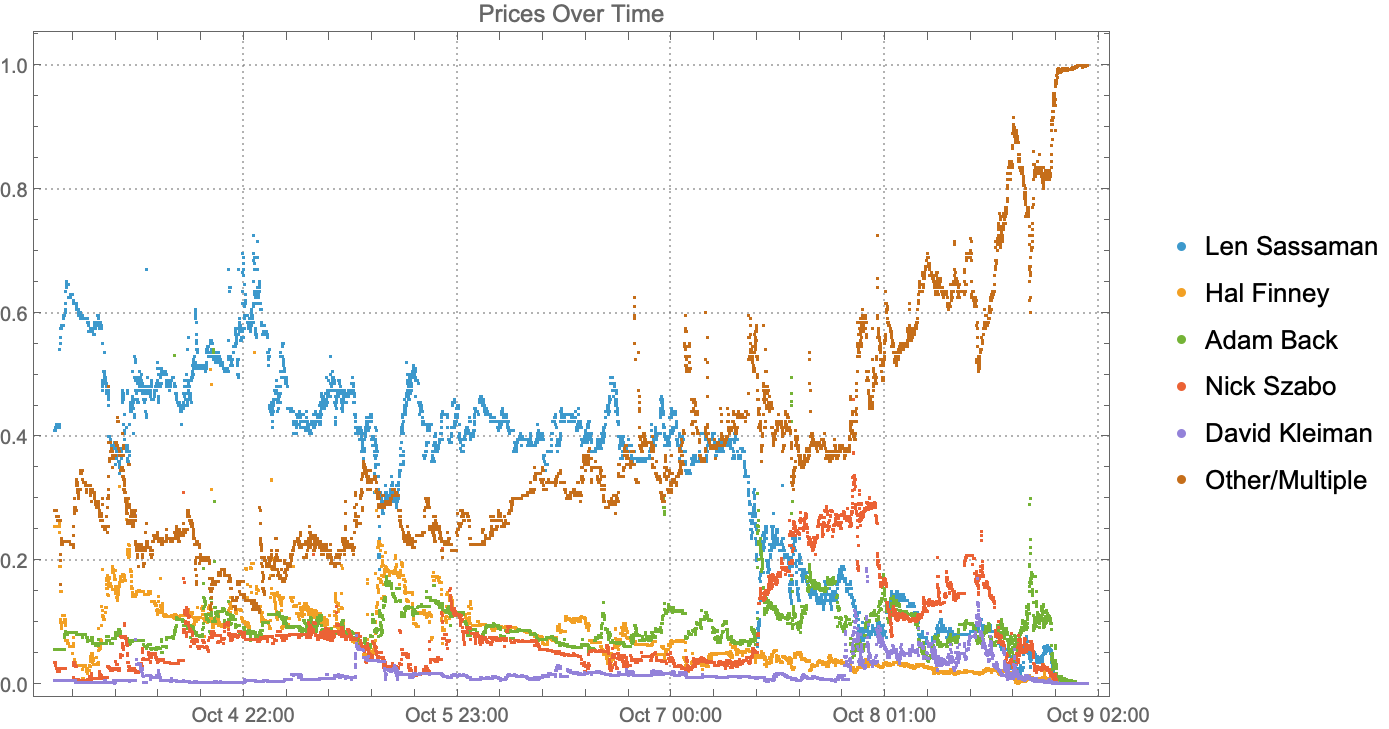
\includegraphics[width=\textwidth]{figures/graph.png}
  \caption{The price movements for 6 leading candidates in the Polymarket market for who would be named as Satoshi Nakamoto in the HBO documentary `Money Electric' which aired the evening of October 8.}
  \label{fig:example}
\end{figure}

\section{Example instantiation of definition}
\label{app:example}

In section~\ref{sec:hbo}, we discussed an example market concerning who the HBO documentary `Money Electric' would name as Satoshi Nakamoto. In this section, we will see how this fits the definitions of a market, prediction market system, and the Arrow--Debreau special case. As discussed in Section~\ref{wf:mech}, Polymarket employs a market mechanism we call a yes/no bundle (YNB), as opposed to winner-take-all (WTA). YNB requires an extra step in the definitions so we will do a first pass with a simplified WTA submarket, and then add the full YNB market.

\subsection{Pass 1: Single WTA Market}

Consider a simplified market that questions whether one specific candidate, \eg Hal Finney, is named as Satoshi: yes or no. If through unforeseen circumstances, who the documentary names is not verifiable by the air date, the market resolves to no.

Recall Definition~\ref{def:market} of a market: 

\begin{definition}[Market]
A (single) market is a tuple $M=(E,\Omega,J,R)$, where $E$ is a well-defined uncertain event, $\Omega$ is a nonempty outcome space for $E$, $J$ is a finite index set of contract labels (“shares”), and $R=(R_j)_{j\in J}$ are nonnegative payoff functions with $R_j:\Omega\to\mathbb{R}_{\ge 0}$. 
We assume $|J|\ge|\Omega|$ and we require \emph{outcome distinguishability} on $\Omega$:
\[
\forall\,\omega\neq\omega'\in\Omega\ \ \exists\,j\in J:\ R_j(\omega)\neq R_j(\omega').
\]
When $M$ resolves to $\omega_M\in\Omega$, one unit of share $j\in J$ pays $R_j(\omega_M)$ (in units of $\mathcal{N}$ defined below).
\end{definition}

Event $E$ is whether or not Hal Finney is named as Satoshi in the documentary.

$\Omega$ is the set of resolution outcomes the market recognizes for $E$—the labels the system can publish at settlement. For this Hal-only binary market the outcome space is $\Omega=\{\mathsf{True},\mathsf{False}\}$. Here $\mathsf{True}$ means the documentary (per the market’s stated criteria) identifies Hal Finney as Satoshi; $\mathsf{False}$ aggregates all other possibilities (Hal not named, someone else named, no one named, the film does not air, or the identification is not verifiable by the resolution deadline).

%Once some $\omega\in\Omega$ is published, all payoffs $R_j(\omega)$ are determined.

We require that $\Omega$ contain no redundant labels. A label is redundant if it does not change at least one contract’s payoff: $\omega\sim\omega' \iff \forall j\in J,\ R_j(\omega)=R_j(\omega')$. For example, “Hal is named and it is raining’’ and “Hal is named and it is not raining’’ are distinct real-world states, but they cannot both appear in $\Omega$ since they both map to $\mathsf{True}$. The restriction can be written as:
\[
\forall\,\omega\neq\omega'\in\Omega\ \ \exists\,j\in J:\ R_j(\omega)\neq R_j(\omega').
\]

In a prediction market, there are a set of shares. If we label them and add them all to an index set, that set is $J$. For this example, $J=\{\textsf{YES},\textsf{NO}\}$: Hal Finney is named (yes) and else (no). This is a normal case where each share in $J$ corresponds to an outcome in $\Omega$ but it is possible that the number of shares could exceed the number of outcomes.\footnote{For example, consider a market of where Newcastle United (NUFC) finishes in the 2024-35 English Premier League season. Since there are 20 teams, the outcome has 20 possible labels: positions 1 to 20. Shares could exist for each of the 20 positions. But the outcome could also settle shares for whether NUFC finishes in the top 5 (which is relevant to champions league admittance), or shares on finishing in the bottom 3 (which is relevant to relegation).}

$J$ is the index set of contract labels—the names of the tradeable shares. In this binary market we take $J=\{\textsf{YES},\textsf{NO}\}$. 

The labels get their meaning from the component payoff functions $R_j:\Omega\to\mathbb{R}_{\ge 0}$. In this example, a payoff of 1 is given for shares that correctly predict the outcome and 0 otherwise. This means $R_{\textsf{YES}}(\mathsf{True})=1$, $R_{\textsf{YES}}(\mathsf{False})=0$, $R_{\textsf{NO}}(\mathsf{True})=0$, $R_{\textsf{NO}}(\mathsf{False})=1$.

Recall Definition~\ref{def:market} of a prediction--market system $\mathcal{S}=(\mathcal{M},\mathcal{N},\mathsf{Res})$:
$\mathcal{M}$ is the (countable) catalog of markets; $\mathcal{N}$ is the numeraire (unit of account used to price and settle claims);
and $\mathsf{Res}=\{\mathrm{res}_M\}_{M\in\mathcal{M}}$ assigns to each market $M$ a resolution register that is initially
$\bot$ and flips exactly once to some $\omega_M\in\Omega_M$.
When $\mathrm{res}_M\neq\bot$, we set $\omega_M:=\mathrm{res}_M$ and each unit of label $j\in J$ settles for $R_j(\omega_M)$ units of $\mathcal{N}$.

This market is a winner--take--all (Arrow--Debreu) special case: there is a bijection $\iota:J\to\Omega$ as follows: $\textsf{YES}\rightarrow\mathsf{True}$ and $\textsf{NO}\rightarrow\mathsf{False}$. Payoffs are $R_j(\omega)=\mathbf{1}\{\omega=\iota(j)\}$. Hence, for each $\omega\in\Omega$, exactly one label pays $1$ and all others pay $0$. 

The market tuple $M=(E,\Omega,J,R)$ specifies \emph{what} to pay \emph{given} an outcome (via $R$).
The register $\mathrm{res}_M$ is the system’s single source of truth for \emph{which} outcome actually occurred:
before resolution $\mathrm{res}_M=\bot$ (no settlement), after resolution $\mathrm{res}_M=\omega_M\in\Omega_M$ (settlement applies).

Polymarket instantiates $\mathcal{S}$ with $\mathcal{M}$ equal to its live and historical markets, $\mathcal{N}$ the USD–denominated stablecoin USDC, and $\mathsf{Res}$ implemented by its on–chain resolution process (e.g., UMA’s optimistic oracle) that writes a single outcome to each $\mathrm{res}_M$.

For the Hal–only binary market, the system maintains a resolution register
$\mathrm{res}_{M_{\mathrm{Hal}}}\in\{\bot\}\cup\Omega$ with
$\Omega=\{\mathsf{True},\mathsf{False}\}$ (i.e., “yes/no” to the proposition).
The register is initially $\bot$ and, after the platform’s resolution process completes, the oracle writes a single value
$\omega_{M_{\mathrm{Hal}}}\in\Omega$ to the register.

Set $\omega_{M_{\mathrm{Hal}}}=\mathsf{True}$ iff the documentary (per stated criteria) identifies \emph{Hal Finney} as Satoshi; otherwise set $\omega_{M_{\mathrm{Hal}}}=\mathsf{False}$.

Shares are fully collateralized to \$1 in the numeraire $\mathcal{N}$ (USDC): a unit of \textsf{YES} pays $1$\,USDC at $\mathsf{True}$ and $0$\,USDC at $\mathsf{False}$; a unit of \textsf{NO} pays $1$\,USDC at $\mathsf{False}$ and $0$\,USDC at $\mathsf{True}$. Formally,
\[
R_{\textsf{YES}}(\mathsf{True})=1,\ \ R_{\textsf{YES}}(\mathsf{False})=0,\qquad
R_{\textsf{NO}}(\mathsf{True})=0,\ \ R_{\textsf{NO}}(\mathsf{False})=1.
\]

In the aired documentary, \emph{Peter Todd} was named; therefore
\[
\mathrm{res}_{M_{\mathrm{Hal}}}=\omega_{M_{\mathrm{Hal}}}=\mathsf{False},
\]
and each unit settles as
\[
\textsf{YES}\ \to\ 0\ \text{USDC},\qquad
\textsf{NO}\ \to\ 1\ \text{USDC}.
\]

% = = = 

\subsection{Pass 2: YNB Market}

We define a \textit{family} of markets $\{M_c\}_{c\in C}$ where each $c\in C$ names one market in the family. For the HBO film, $C$ is the set of candidates including $\mathsf{Finney}$, $\mathsf{Szabo}$,  $\mathsf{Sassaman}$,  $\mathsf{Back}$, and $\mathsf{Other/Multiple}$. The event $E_c$ for a particular $\{M_c\}$ is: the documentary identifies $c$ as Satoshi. For each candidate's market, the relevant market outcomes are $\Omega_c=\tuple{\mathsf{True},\mathsf{False}}$. As a YNB market, Polymarket creates a yes share and a no share for each candidate $J_c=\tuple{\textsf{YES},\textsf{NO}}$ called a yes/no bundle (YNB). The payoffs are as follows: $R^{(c)}_{\textsf{YES}}(\mathsf{True})=1$, $R^{(c)}_{\textsf{YES}}(\mathsf{False})=0$, $R^{(c)}_{\textsf{NO}}(\mathsf{True})=0$, and $R^{(c)}_{\textsf{NO}}(\mathsf{False})=1$. Each $\{M_c\}$ has its own volume of outstanding shares, its own pricing, and its own orderbook or AMM. 

For settling, $\mathsf{Res}=\{\mathrm{res}_{M}\}_{M\in\mathcal{M}}$ gives each $M_c$ a register $\mathrm{res}_{M_c}\in\{\bot\}\cup\Omega_c$, initially $\bot$, that flips exactly once to $\omega_{M_c}\in\Omega_c$. The documentary named Peter Todd, who was not one of the named candidates and thus fell under \textsf{Other/Multiple}: $\omega_{M_{\textsf{Other/Multiple}}}=\mathsf{True}$ while $\omega_{M_c}=\mathsf{False}$ for all other $c\neq\textsf{Other/Multiple}$. 

The $R^{(c)}_j(\omega_{M_c})$ for \textsf{Other/Multiple: YES} was $1$ USDC, \textsf{Other/Multiple: NO} was $0$ USDC, every other named candidate’s \textsf{NO} paid $1$ USDC and their corresponding \textsf{YES} paid $0$ USDC. 

% = = = 

\subsection{Axioms}

Polymarket works through \textit{splitting} (see \S\ref{wf:trade}) as follows. Any trader can receive 1 yes share and 1 no share for a specified candidate's market $\{M_c\}$  by depositing 1 USDC into the treasury for the market. When the market resolves, one share will resolve for 1 USDC and one will resolve for 0 USDC. Thus in both cases, Polymarket has exactly the correct amount in the treasury to complete its payout and is solvent. Every split increases the number of shares (yes and no) by 1 share and increase the treasury by 1 USDC. After the market resolves, the winning shares can be redeemed for 1 USDC which decreases the outstanding winning shares by 1 and reduces the treasury by 1 USDC. Shares are fungible as the payout for each share of the same type is identical. Polymarket allows shares to withdrawn as ERC20 tokens and traded using any compatible marketplace. It also provides a CLOB and an AMM for each share.

The HBO documentary market is a special case, called negative risk (NR), in which each candidate's yes/no bundle is a complete set of outcomes (either the candidate is named or the candidate is not named) and additionally the set of yes shares for each candidate is complete (one and only one of the candidates will be declared the winner). Thus it is WTA across each yes/no bundle and it is also WTA across all yes shares.



\end{document}







